% Versão 24/06/2020

% Este documento destina-se a servir como modelo para a produção de documentos
% de pesquisa do PPGINF/UFPR, como projetos, dissertações e teses. A classe de
% documento se chama "ppginf" (arquivo ppginf.cls) e define o formato básico do
% documento. O texto está organizado em capítulos que são colocados em
% subdiretórios separados. São definidos exemplos para a inclusão de figuras,
% códigos-fonte e a definição de tabelas.
%
% Produzido por Carlos Maziero (maziero@inf.ufpr.br).

%=====================================================

% Opções da classe ppginf:
%
% - defesa    : versão para entregar à banca; tem espaçamento 1,5
%               e omite algumas páginas iniciais (agradecimentos, etc)
% - final     : versão pós-defesa, para enviar à biblioteca;
%               tem espaçamento simples e todas as páginas iniciais.
% - oneside   : somente frente; use quando for gerar somente o PDF.
% - twoside   : frente/verso; use se precisar de uma versão impressa.
% - metadados : inclui metadados no PDF (por default não inclui)
% - ...       : demais opções aceitas pela classe "book"

% ATENÇÂO: este modelo tem suporte para português e inglês.
% As duas línguas devem ser informadas como opção da classe;
% a língua principal do documento deve vir POR ÚLTIMO.

% Versão para a defesa (português)
\documentclass[defesa,oneside,english,brazilian]{ppginf}

% Versão para a defesa (inglês)
%\documentclass[defesa,oneside,brazilian,english]{ppginf}

% Versão final para a biblioteca da UFPR (português)
%\documentclass[final,oneside,english,brazilian]{ppginf}

% Versão final para a biblioteca da UFPR (inglês)
%\documentclass[final,oneside,brazilian,english]{ppginf}

% Versão final para impressão (frente/verso, português)
%\documentclass[final,twoside,english,brazilian]{ppginf}

% Versão final para impressão (frente/verso, inglês)
%\documentclass[final,twoside,brazilian,english]{ppginf}

% configurações de diversos pacotes, inclusive a fonte usada no texto
% Pacotes usados neste documento e suas respectivas configurações

% ------------------------------------------------------------------------------

% Definição de fontes

% formato dos arquivos-fonte (utf8 no Linux e latin1 no Windows)
\usepackage[utf8]{inputenc}	% arquivos LaTeX em Unicode (UTF8)

% usar codificação T1 para ter caracteres acentuados corretos no PDF
\usepackage[T1]{fontenc}

% fonte usada no corpo do texto (pode alterar, mas descomente apenas uma)
\usepackage{newtxtext,newtxmath}	% Times (se não tiver, use mathptmx)
%\usepackage{lmodern}			% Computer Modern (fonte clássico LaTeX)
%\usepackage{kpfonts}			% Kepler/Palatino (idem, use mathpazo)
%\renewcommand{\familydefault}{\sfdefault} % Arial/Helvética (leia abaixo)

% A biblioteca central da UFPR recomenda usar Arial, seguindo a recomendação da
% ABNT. Essa é uma escolha ruim, pois fontes sans-serif são geralmente inade-
% quados para textos longos e impressos, sendo melhores para páginas Web.
% http://www.webdesignerdepot.com/2013/03/serif-vs-sans-the-final-battle/.

% fontes usadas em ambientes específicos
\usepackage[scaled=0.9]{helvet}		% Sans Serif
\usepackage{courier}			% Verbatim, Listings, etc

% fontes adicionais
\usepackage{amsmath}		% pacotes matemáticos
\usepackage{amsfonts}		% fontes matemáticas 
%\usepackage{amssymb}		% símbolos 

% ------------------------------------------------------------------------------

% inclusão de figuras em PDF, PNG, PS, EPS
\usepackage{graphicx}

% subfiguras (subfigure is deprecated, don't use it)
\usepackage[labelformat=simple]{subcaption}
\renewcommand\thesubfigure{(\alph{subfigure})}

% ------------------------------------------------------------------------------

% inclusão/formatação de código-fonte (programas)
\usepackage{listings}
\lstset{language=c}
\lstset{basicstyle=\ttfamily\footnotesize,commentstyle=\textit,stringstyle=\ttfamily}
\lstset{showspaces=false,showtabs=false,showstringspaces=false}
\lstset{numbers=left,stepnumber=1,numberstyle=\tiny}
\lstset{columns=flexible,mathescape=true}
\lstset{frame=single}
\lstset{inputencoding=utf8,extendedchars=true}
\lstset{literate={á}{{\'a}}1  {ã}{{\~a}}1 {à}{{\`a}}1 {â}{{\^a}}1
                 {Á}{{\'A}}1  {Ã}{{\~A}}1 {À}{{\`A}}1 {Â}{{\^A}}1
                 {é}{{\'e}}1  {ê}{{\^e}}1 {É}{{\'E}}1  {Ê}{{\^E}}1
                 {í}{{\'\i}}1 {Í}{{\'I}}1
                 {ó}{{\'o}}1  {õ}{{\~o}}1 {ô}{{\^o}}1
                 {Ó}{{\'O}}1  {Õ}{{\~O}}1 {Ô}{{\^O}}1
                 {ú}{{\'u}}1  {Ú}{{\'U}}1
                 {ç}{{\c{c}}}1 {Ç}{{\c{C}}}1 }

% ------------------------------------------------------------------------------

% formatação de algoritmos
\usepackage{algorithm,algorithmic}
\IfLanguageName{brazilian} {\floatname{algorithm}{Algoritmo}}{}
\renewcommand{\algorithmiccomment}[1]{~~~// #1}
%\algsetup{linenosize=\footnotesize,linenodelimiter=.}

% ------------------------------------------------------------------------------

% formatação de bibliografia (escolher UM estilo e comentar os demais)

% 1: estilo Apalike + Natbib (recomendo usar este!)
\usepackage{natbib}			% bibliografia no estilo NatBib
\IfLanguageName{brazilian}
{\bibliographystyle{apalike-ptbr}}	% formato em português
{\bibliographystyle{apalike}}		% formato em inglês
\renewcommand{\cite}{\citep}		% \cite deve funcionar como \citep

% 2: estilo apacite (ATENÇÃO: ainda não tem suporte para português)
%\usepackage[natbibapa]{apacite}
%\bibliographystyle{apacite}

% 3: outros estilos de bibliografia recomendados
% Mais infos: https://pt.sharelatex.com/learn/Bibtex_bibliography_styles
%
%\bibliographystyle{alpha}		% [Maz06]
%\bibliographystyle{plainnat}		% vide Google "LaTeX Natbib"
%\bibliographystyle{plain}		% [1] ordem alfabética
%\bibliographystyle{unsrt}		% [1] ordem de uso no texto
% no estilo "unsrt", evita que citações nos índices sejam consideradas
%\usepackage{notoccite}

%\bibpunct{[}{]}{;}{a}{}{,}	% caracteres usados nas referências

% ------------------------------------------------------------------------------

% pacotes diversos
\usepackage{alltt,moreverb}	% mais comandos no modo verbatim
\usepackage{currfile}		% infos sobre o arquivo/diretório atual
\usepackage[final]{pdfpages}	% inclusão de páginas em PDF
\usepackage{longtable}		% tabelas multi-páginas (tab símbolos/acrônimos)
\usepackage{booktabs}

% ------------------------------------------------------------------------------


% ------------------------------------------------------------------------------
% 2026-10-29 (parecer de orientação, §7): ABNT/SiBi
% - "Quadro" para conteúdo não numérico, com lista própria;
% - "Fonte:" abaixo de cada ilustração e tabela (título acima).
\usepackage{newfloat}
\DeclareFloatingEnvironment[fileext=loq,listname={Lista de quadros},name=Quadro,placement=htbp,within=chapter]{quadro}
\newcommand{\fonte}[1]{\par\vspace{2pt}{\footnotesize Fonte: #1\par}}
\newcommand{\fonteautor}{\fonte{o autor (2026).}}


% Números dos experimentos: \result{chave} vem de ../generated (gerado por
% experiments/export_paper.sh). Uma chave inexistente interrompe a compilação.
\makeatletter
\def\input@path{{./}{../}}
\makeatother
\graphicspath{{./}{../}}
\input{generated/results}
% vírgula decimal no texto em português; \resulten mantém o ponto (abstract)
\usepackage{xstring}
\let\resulten\result
\makeatletter
\renewcommand{\result}[1]{\@ifundefined{result@#1}%
  {\PackageError{results}{Unknown result key `#1'}{Run the experiment, then experiments/export_paper.sh.}}%
  {{\StrSubstitute{\csname result@#1\endcsname}{.}{{,}}}}}% grupo: o xstring não engole o espaço seguinte
\makeatother

%=====================================================

\begin {document}

% Principais dados, usados para gerar as páginas iniciais.
% Campos não utilizados podem ser removidos ou comentados.

% título
% Pendente (orientador): idioma do documento. Título em inglês com texto em português;
% ou tudo em português, ou tudo em inglês com resumo e folha de rosto em português.
% 2026-10-30 (análise crítica, F2): "Expression-Preserving" removido; o erro de expressão é
% 4,6x o piso de ruído e empata com o GANonymization. "Synthetic identity swap": os pixels
% mostrados vêm da troca (inswapper + GFPGAN); a difusão só gera a identidade-fonte.
\title{Lose the Faces, Keep the Lesson: Face De-Identification of Classroom Video by Synthetic Identity Swap}

% palavras-chave e keywords (p/ resumo, abstract e metadados do PDF)
% 2026-10-29: separadas por ";" e em minúsculas (NBR 6028); "desidentificação", não "anonimização" (LGPD art. 12)
\pchave{desidentificação facial; modelos de difusão; privacidade; vídeo educacional; LGPD}
\keyword{face de-identification; diffusion models; privacy; classroom video; LGPD}

% autoria
\author{Ludwig Aumann}
\advisor{Prof. Dr. Eduardo Todt}

% instituição
\IfLanguageName{brazilian}
  { \instit{UFPR}{Universidade Federal do Paraná} }
% a Bib/UFPR exige que tudo seja em português, exceto o título :-(
%  { \instit{UFPR}{Federal University of Paraná} }
  { \instit{UFPR}{Universidade Federal do Paraná} }

% área de concentração (default do PPGInf, não mudar)
\IfLanguageName{brazilian}
  { \field{Computação} }
% a Bib/UFPR exige que tudo seja em português, exceto o título :-(
%  { \field{Computer Science} }
  { \field{Computação} }

% data (só o ano)
\date{2026}

% local
\IfLanguageName{brazilian}
  { \local{Curitiba PR} }
% a Bib/UFPR exige que tudo seja em português, exceto o título :-(
%  { \local{Curitiba PR - Brazil} }
  { \local{Curitiba PR} }

% imagem de fundo da capa (se não desejar, basta comentar)
\coverimage{0-iniciais/fundo-capa.png}

%=====================================================

%% Descrição do documento (obviamente, descomentar somente UMA!)

% Por exigência da biblioteca da UFPR, a descrição do documento deve ser
% em português, mesmo em documentos em outras línguas. Vá entender...

% 2026-10-29: texto do modelo SiBi/UFPR para TCC
\descr{Trabalho de Conclusão de Curso apresentado ao curso de Graduação em Ciência da Computação, Setor de Ciências Exatas, Universidade Federal do Paraná, como requisito parcial à obtenção do título de Bacharel em Ciência da Computação}

% exame de qualificação de doutorado
%\descr{Documento apresentado como requisito parcial ao exame de qualificação de Doutorado no Programa de Pós-Graduação em Informática, Setor de Ciências Exatas, da Universidade Federal do Paraná}

% dissertação de mestrado
%\descr{Dissertação apresentada como requisito parcial à obtenção do grau de Mestre em Informática no Programa de Pós-Graduação em Informática, Setor de Ciências Exatas, da Universidade Federal do Paraná}

% exame de qualificação de mestrado
%\descr{Documento apresentado como requisito parcial ao exame de qualificação de Mestrado no Programa de Pós-Graduação em Informática, Setor de Ciências Exatas, da Universidade Federal do Paraná}

% trabalho de conclusão de curso
%\descr{Trabalho apresentado como requisito parcial à conclusão do Curso de Bacharelado em XYZ, Setor de Ciências Exatas, da Universidade Federal do Paraná}

% trabalho de disciplina
%\descr{Trabalho apresentado como requisito parcial à conclusão da disciplina XYZ no Curso de Bacharelado em XYZ, Setor de Ciências Exatas, da Universidade Federal do Paraná}

% doctorate thesis
%\descr{Thesis presented as a partial requirement for the degree of Doctor in Computer Science in the Graduate Program in Informatics, Exact Sciences Sector, of the Federal University of Paraná, Brazil}

% doctorate qualification
%\descr{Document presented as a partial requirement for the doctoral qualification exam in the Graduate Program in Informatics, Exact Sciences Sector, of the Federal University of Paraná, Brazil}

% MSc dissertation
%\descr{Dissertation presented as a partial requirement for the degree of Master of Sciences in Informatics in the Graduate Program in Informatics, Exact Sciences Sector, of the Federal University of Paraná, Brazil.}

% MSc qualification
%\descr{Document presented as a partial requirement for the Master of Sciences qualification exam in the Graduate Program in Informatics, Exact Sciences Sector, of the Federal University of Paraná, Brazil}

%=====================================================

% define estilo das páginas iniciais (capas, resumo, sumário, etc)
\frontmatter
\pagestyle{frontmatter}

% produz capa e folha de rosto
\titlepage

% páginas que só aparecem na versão final (a inclusão é automática)
% % IMPORTANTE: o conteúdo exato da ficha catalográfica é preparada pela
% Biblioteca da UFPR. Não "invente" um conteúdo para ela!

\begin{ficha}	% só gera conteúdo se for na versão final

% inclusão da ficha catalográfica final (arquivo PDF)
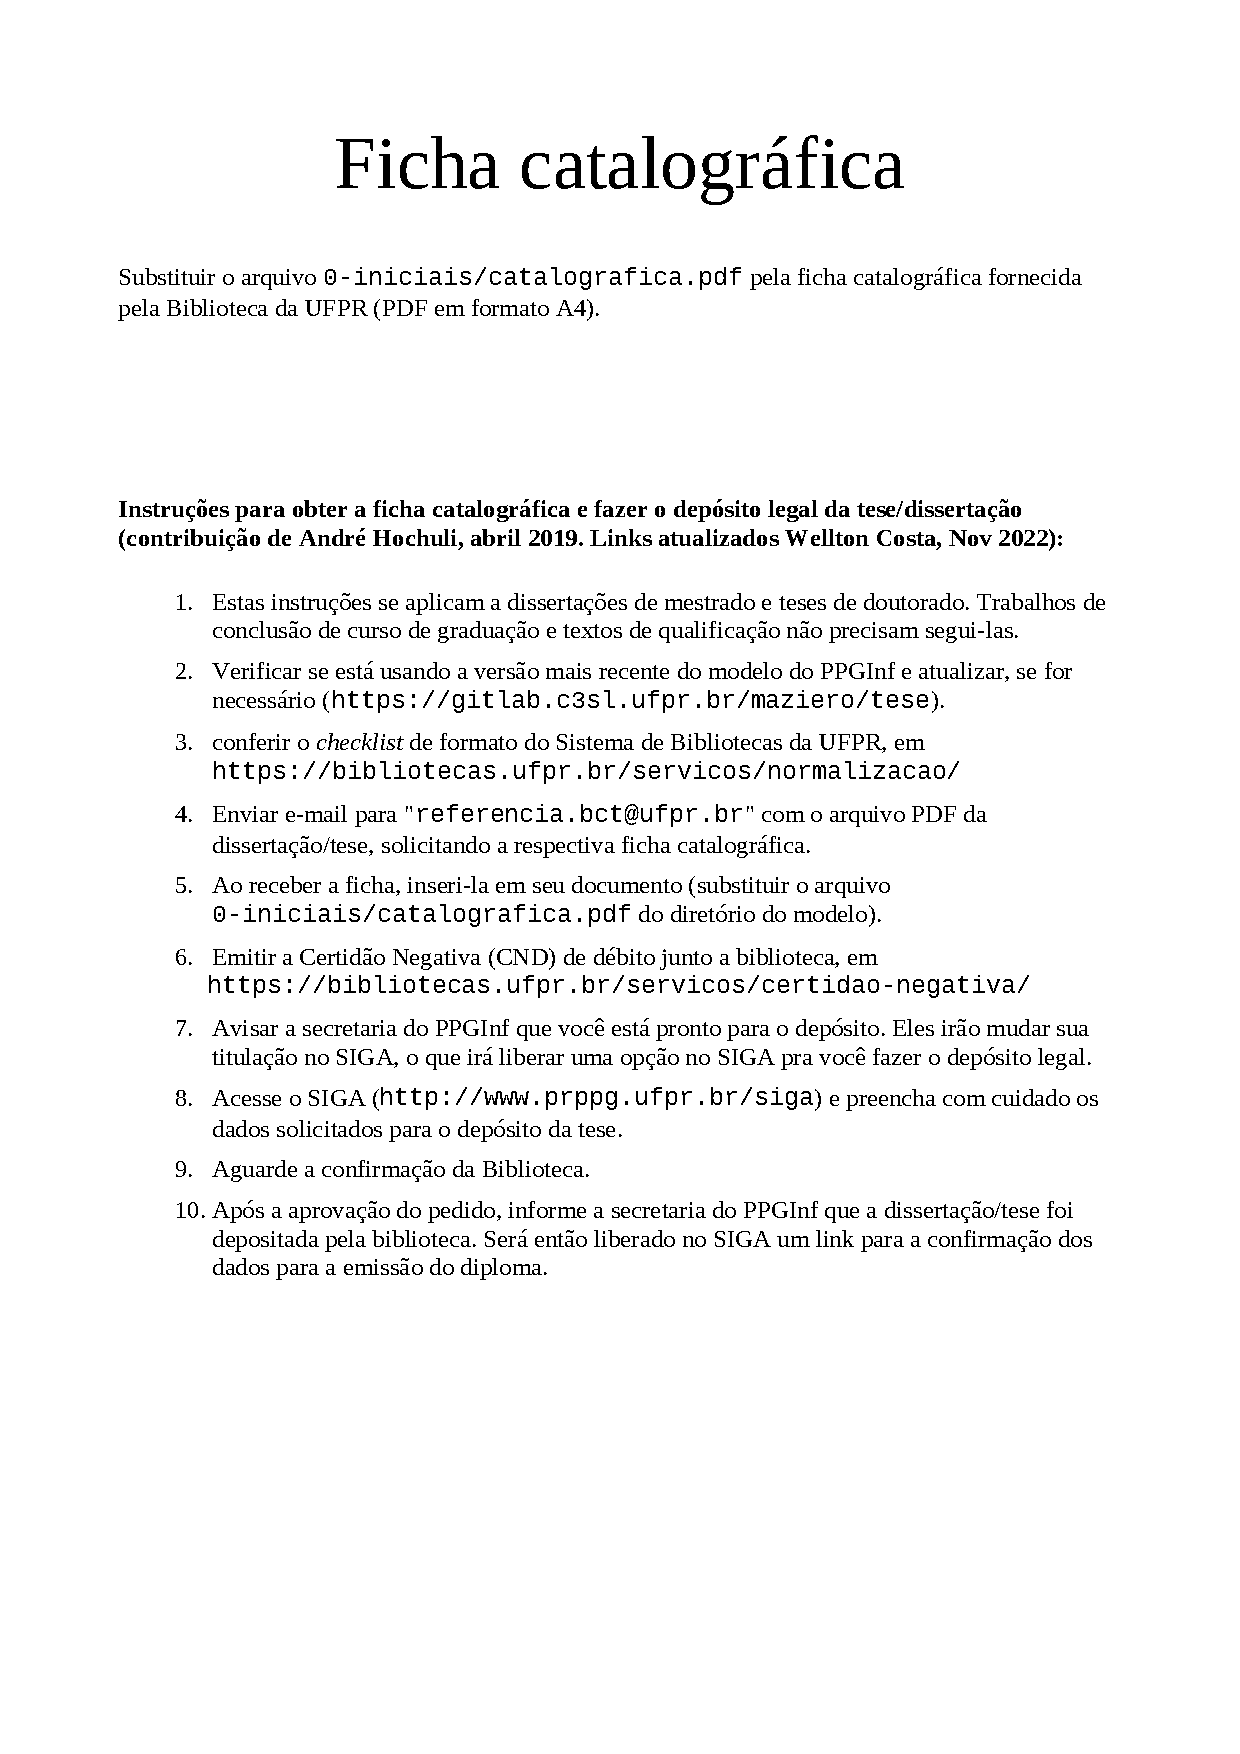
\includepdf[noautoscale]{0-iniciais/catalografica.pdf}

\end{ficha}

%=====================================================
	% ficha catalográfica: não exigida para TCC (2026-10-29)
% A ficha de aprovação será fornecida pela secretaria do programa,
% após a defesa e cumprimento dos demais trâmites legais.

\begin{aprovacao}	% só gera conteúdo se for na versão final

% inclusão do termo de aprovação final (arquivo PDF)
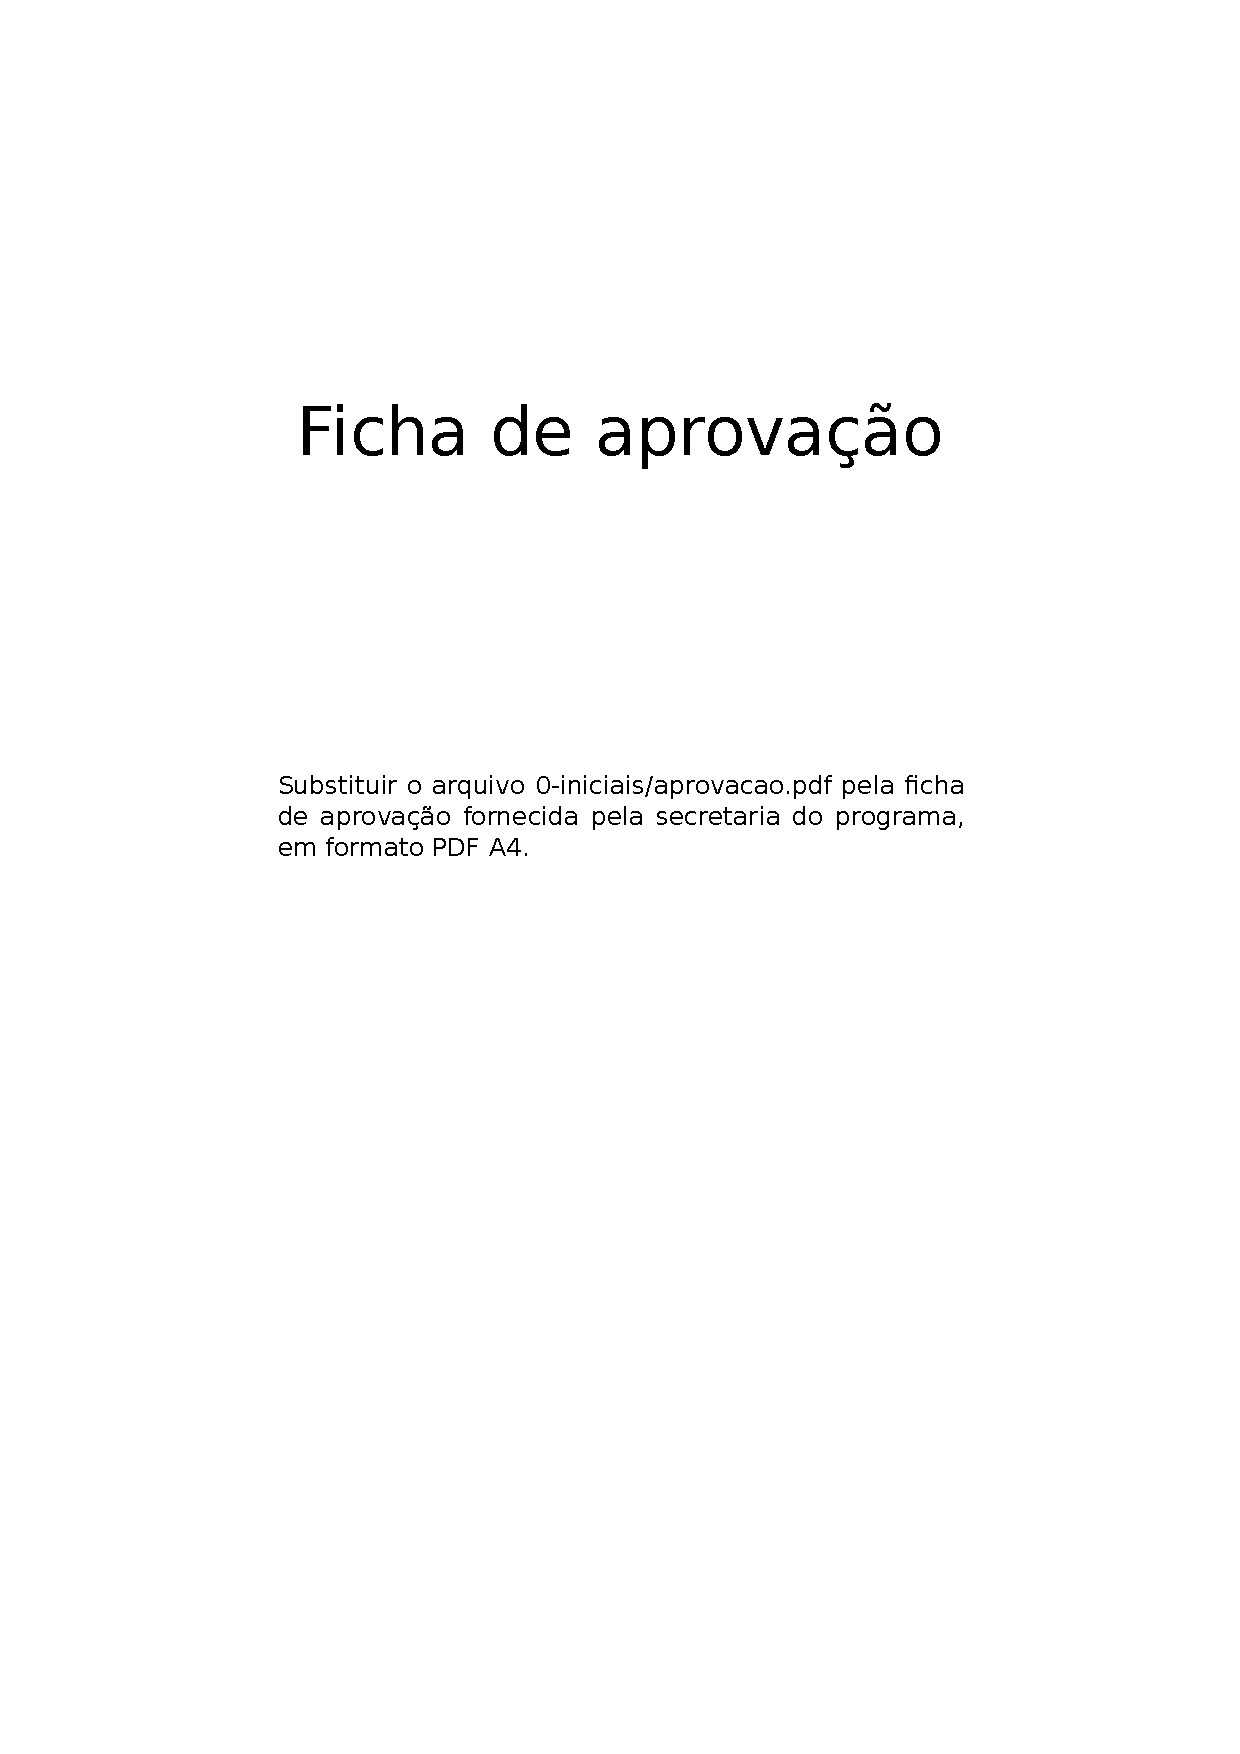
\includepdf[noautoscale]{0-iniciais/aprovacao.pdf}

\end{aprovacao}

%=====================================================
		% folha de aprovação
\begin{dedica}  % só gera conteúdo se for na versão final

% Pendente (autor); opcional. 2026-10-29: texto do modelo removido.
Pendente.

\end{dedica}
		% dedicatória
\begin{agradece}	% só gera conteúdo se for na versão final

% Pendente (autor): texto dos agradecimentos, no máximo uma página.
% 2026-10-29: \lipsum do modelo removido (parecer de orientação, §3.3).
Pendente.

\end{agradece}
		% agradecimentos

% resumo (português) e abstract (inglês)
\begin{resumo}

% Rascunho factual (2026-10-22), revisado em 2026-10-29 (parecer de orientação) e em
% 2026-10-30 (análise crítica):
% - parágrafo único, 3ª pessoa, objetivo → método → resultados → conclusão (NBR 6028);
% - alegação: desidentificação facial, não anonimização (LGPD art. 12; Seção~\ref{sec:ameaca});
% - substituição híbrida: difusão só na identidade-fonte; pixels da troca de rosto (F2);
% - ponto de operação β 1,2 (não o braço mais forte); custo em emoção explícito (G6);
% - comparação pelo par (rank-1 entre rostos com face sintética, parcela coberta): o
%   rank-1 do vídeo final premia ocultar (F1).
Vídeos de sala de aula expõem a identidade de alunos e professores. Este
trabalho investiga se trocar cada rosto detectado por uma identidade sintética
reduz a reidentificação facial automática e mantém o sinal comportamental
(expressão, pose, emoção), medido no vídeo que o espectador vê. O pipeline é
híbrido e tem três estágios: detecção SCRFD-10GF com rastreamento e um pós-passe
de recall; uma identidade sintética Stable Diffusion XL por track, trocada no
rosto de cada quadro por \texttt{inswapper} com restauração GFPGAN; e composição
\emph{fail-closed}, que oculta todo rosto detectado sem substituição válida. A
contribuição principal empurra o embedding de identidade usado pela troca para
longe da identidade real estimada no track. Em três vídeos curtos (29\,s no
total), no ponto de operação escolhido, o rank-1 do FaceNet, reconhecedor não
usado na otimização, cai de \result{e3c/pooled/native/facenet.rank1} para
\result{e3c/pooled/b-1.2/facenet.rank1}, sem diferença mensurável em expressão e
pose e com queda não significativa da concordância de emoção
(\result{e3c/pooled/native/emotion_kappa} para \result{e3c/pooled/b-1.2/emotion_kappa}).
Entre os rostos que recebem face sintética, o pipeline final é reidentificado em
\result{derived/frontier/e5-ref/rank1} cobrindo \result{derived/frontier/e5-ref/share}
dos rostos, contra \result{derived/frontier/e2-blanket/rank1} do BLANKET liberado,
que cobre \result{derived/frontier/e2-blanket/share}; no vídeo final, porém,
métodos que ocultam mais rostos têm rank-1 menor, e borramento, mosaico e GANs
têm rank-1 menor que o do pipeline. Orientação por gradiente no amostrador de difusão e
otimização do código de identidade de uma rede adversarial generativa não têm
efeito mensurável. O erro de expressão fica em
\result{e3e/pooled/gate/expression} unidades de distância interocular, cerca de
quatro vezes o piso de ruído, e nenhum método preserva a emoção. O custo projetado
do laço por rosto é de \result{e5/pooled/adapt-0.08/class-hours} horas de unidade
de processamento gráfico (GPU) por hora de aula. O resultado é desidentificação
facial parcial, outro ponto do compromisso entre privacidade, cobertura e
utilidade, e não anonimização: cabelo, contorno da cabeça, roupa e voz permanecem.

\end{resumo}

\begin{abstract}

% Factual draft (2026-10-22), revised 2026-10-29: translation of the resumo,
% third person, no internal labels, de-identification rather than anonymization.
Classroom recordings expose students' and teachers' identities. This work
investigates whether replacing every detected face with a synthetic one reduces
automatic face re-identification while keeping behavioral signal (expression,
pose, emotion), measured on the video a viewer sees. The pipeline has three
stages: SCRFD-10GF detection with tracking and a recall post-pass; replacement
with BLANKET (one Stable Diffusion XL synthetic identity per track and an
\texttt{inswapper} face swap per frame); and fail-closed composition, which hides
every known face that has no valid replacement. The main contribution pushes the
swap's identity embedding away from the track's estimated real identity. On three
short videos (29\,s in total), held-out FaceNet rank-1 drops from
\resulten{e3c/pooled/native/facenet.rank1} to
\resulten{e3c/pooled/b-1.6/facenet.rank1} with no measurable expression or pose
cost; the direction of the effect holds when the push strength is chosen without
the evaluated video. With a privacy filter the final video reaches
\resulten{e3e/pooled/gate/facenet_final.rank1}, between
\resulten{derived/gate-final/x-chance-min} and
\resulten{derived/gate-final/x-chance-max} times chance depending on the video,
against \resulten{e2/pooled/blur/facenet_final.rank1} for blur, which erases
behavior. Gradient guidance inside the diffusion sampler and identity-code
optimization in a generative adversarial network have no measurable effect.
Running the main process on the GPU and adaptive frame sampling bring the
projected per-face loop cost to \resulten{e5/pooled/adapt-0.08/class-hours} GPU
hours per hour of class. No method keeps emotion near its noise floor. The
result is partial face de-identification, another point on the privacy--utility
trade-off, not anonymization: hair, head outline, clothing and voice remain.

\end{abstract}


% listas  de figuras, tabelas, abreviações/siglas, símbolos
\listoffigures				% figuras
\clearpage
\listoftables				% tabelas
\clearpage
\listofquadros				% quadros (2026-10-29)
%=====================================================

% lista de acrônimos (siglas e abreviações)

\begin{listaacron}

\begin{longtable}[l]{p{0.2\linewidth}p{0.7\linewidth}}
AP & \emph{Average Precision} (WIDER FACE)\\
C2 & Identidade real agregada por track (componente deste trabalho)\\
CFG & \emph{Classifier-Free Guidance}\\
FAR & \emph{False Accept Rate}\\
FPPI & Falsos positivos por imagem\\
GAN & \emph{Generative Adversarial Network}\\
GFPGAN & Restaurador facial com \emph{Generative Facial Prior}\\
IOD & Distância interocular\\
LGPD & Lei Geral de Proteção de Dados Pessoais (Lei 13.709/2018)\\
P1 & Orientação ArcFace dentro do amostrador SDXL\\
P2 & Empurrão do embedding de identidade na troca de rosto\\
P3 & Otimização do código de identidade do CIAGAN\\
RPC & \emph{Remote Procedure Call}\\
SDXL & Stable Diffusion XL\\
TAR & \emph{True Accept Rate}\\
UFPR & Universidade Federal do Paraná\\
\end{longtable}

\end{listaacron}

%=====================================================
		% acrônimos, deve ser preenchida à mão
%=====================================================

% lista de símbolos

\begin{listasimb}

\begin{longtable}[l]{p{0.2\linewidth}p{0.7\linewidth}}
$e_{\mathrm{real}}$ & Embedding ArcFace da identidade real (agregado no track)\\
$e_{\mathrm{synth}}$ & Embedding ArcFace da identidade sintética\\
$\hat{e}$ & Embedding usado pela troca após o empurrão P2\\
$\beta$ & Força do empurrão P2\\
$\tau$ & Limiar (\emph{hinge} de P1/P3; amostragem adaptativa)\\
$\kappa$ & Kappa de Cohen (concordância de emoção)\\
$\lambda$ & Peso da penalidade do pseudônimo (P3)\\
$\sigma$ & Confiança mínima no termo de qualidade de detecção\\
$N$ & Número de tracks da galeria (acaso do rank-1 $= 1/N$)\\
\end{longtable}

\end{listasimb}

%=====================================================
		% símbolos, idem
\tableofcontents			% sumário

%=====================================================

% define estilo do corpo do documento (capítulos e apêndices)
\mainmatter
\pagestyle{mainmatter}

% inclusao de cada capítulo, alterar a gosto (do professor de Metodologia)
\chapter{Introdução}
\label{cap:intro}

% Rascunho em tópicos (2026-10-22): fatos e decisões, para desenvolver em parágrafos.

\section{Problema}
\begin{itemize}
\item Gravações de aula são evidência para pesquisa educacional: interação, afeto, turnos de fala.
\item As mesmas gravações identificam alunos (muitos menores) e professores.
\item Rosto é dado biométrico; origem racial ou étnica é dado sensível \citep[art.~5, II; art.~11]{lgpd}.
\item Dados de crianças e adolescentes exigem consentimento específico de um dos pais \citep[art.~14, §1º]{lgpd}.
\item Dado anonimizado deixa de ser pessoal, salvo se a anonimização puder ser revertida com esforços razoáveis \citep[art.~12]{lgpd}.
\item Blur e mosaico removem a identidade e também o comportamento (expressão, pose, emoção).
\end{itemize}

\section{Pergunta}
\begin{itemize}
\item Substituir cada rosto por um rosto sintético reduz a reidentificação e mantém o sinal comportamental?
\item Medido no vídeo que o espectador vê, não só nos rostos que o método escolhe substituir.
\end{itemize}

\section{Hipótese original e o que os dados mostraram}
\begin{itemize}
\item Hipótese da proposta: substituição por difusão, demograficamente similar, (a) reduz a similaridade de identidade abaixo de um limiar estrito e (b) preserva emoção e expressão dentro de uma margem aceitável.
\item (a) Parcial: a reidentificação cai, mas não chega ao acaso nem abaixo do blur (Cap.~\ref{cap:resultados}).
\item (b) Parcial: expressão e pose preservadas melhor que em censura e GANs; emoção não chega perto do piso de ruído.
\item Meta pré-definida ``rank-1 $\le 2\times$ o acaso'': não atingida.
\item Resultado: outro ponto do compromisso privacidade--utilidade, não dominância.
\end{itemize}

\section{Contribuições}
\begin{enumerate}
\item Avaliação que mede o vídeo final: três visões de privacidade (rostos gerados; todos os rostos com passthrough como vazamento; vídeo final) mais a visão do vídeo composto (E5). A ordem dos métodos muda conforme a visão.
\item P2: empurrão do embedding de identidade da troca para longe da identidade real do track; redução monotônica e significativa no FaceNet (avaliador não usado na otimização); medição do quanto o ganho no ArcFace não se transfere para o FaceNet.
\item Pipeline \emph{fail-closed} para vídeo de sala de aula: pós-passe de recall, detecção do Estágio~1 dentro da troca, \emph{privacy gate}, composição que nunca mostra rosto conhecido real.
\item Resultados negativos com diagnóstico: orientação no amostrador SDXL (P1) e no código de identidade do CIAGAN (P3).
\item Estudo de custo (E5): onde o tempo vai, o que cada aceleração custa em privacidade e utilidade.
\end{enumerate}

\section{Escopo}
\begin{itemize}
\item Gravações de aula, câmera fixa, processamento \emph{offline}.
\item Só rosto (não corpo inteiro); áudio fora do escopo.
\item Sem garantia formal de privacidade; atacante ingênuo (sem retreino) \citep{hanisch}.
\item Três vídeos de demonstração; não é um conjunto consentido de crianças.
\end{itemize}

\section{Organização}
\begin{itemize}
\item Cap.~\ref{cap:fundam}: fundamentação e trabalhos relacionados.
\item Cap.~\ref{cap:metodo}: pipeline e componentes.
\item Cap.~\ref{cap:experimentos}: configuração experimental (E0--E5).
\item Cap.~\ref{cap:resultados}: resultados.
\item Cap.~\ref{cap:discussao}: pipeline final e discussão.
\item Cap.~\ref{cap:conclusao}: limitações, ética, trabalhos futuros.
\item Apêndices: licenças, registro de decisões, reprodução.
\end{itemize}
			% introdução
\chapter{Fundamentação e trabalhos relacionados}
\label{cap:fundam}

% Rascunho em tópicos (2026-10-22). Cada item: o que é, o que usamos, o que importa aqui.

\section{Detecção de faces}
\begin{itemize}
\item WIDER FACE: benchmark com subconjuntos \emph{easy}/\emph{medium}/\emph{hard} \citep{widerface}. Outros: LFW \citep{wildface}, FDDB \citep{fddb}.
\item SCRFD: redistribuição de amostras e computação; variantes 0.5--34 GFLOPs \citep{scrfd}.
  \begin{itemize}
  \item O pacote \texttt{buffalo\_l} do InsightFace traz SCRFD-10GF com keypoints (\texttt{det\_10g}), não RetinaFace \citep{insightface}.
  \item AP publicado da variante com keypoints (SCRFD\_10G\_KPS): 95,40 / 94,01 / 82,80; 4,23 M parâmetros.
  \end{itemize}
\item RetinaFace: detector de estágio único com localização multinível \citep{retinaface}.
\item YOLO-FaceV2: escala e oclusão; variante \emph{s} \citep{yolofacev2}.
\item Em sala de aula: RetinaFace e YOLOFace com recall alto em dados de sala de aula \citep{gf-ananda}; YOLOv9 para rostos de crianças \citep{ahmed}.
\item Outros considerados: MogFace \citep{mogface}, ADYOLOv5-Face \citep{adyolov5face}.
\end{itemize}

\section{Rastreamento}
\begin{itemize}
\item ByteTrack: associa primeiro detecções de alta confiança; as de baixa confiança só estendem tracks existentes \citep{bytetrack}.
\item Deep OC-SORT: média móvel exponencial da aparência com peso pela confiança \citep{deepocsort}.
\end{itemize}

\section{Reconhecimento facial}
\begin{itemize}
\item ArcFace: margem angular aditiva \citep{arcface}; usamos \texttt{w600k\_r50} (ResNet-50, WebFace600K, subconjunto de \citealp{webface260m}).
\item FaceNet: embedding por perda tripla \citep{facenet}; usamos InceptionResnetV1 treinado em VGGFace2 \citep{vggface2,facenetpytorch}.
\item Agregação de templates em vídeo ponderada por qualidade: NAN \citep{nan}, QAN \citep{qan}.
\end{itemize}

\section{Anonimização por censura e GAN}
\begin{itemize}
\item Blur e mosaico: removem identidade e comportamento; reversíveis ou atacáveis em rostos pequenos \citep{fantomas}.
\item DeepPrivacy: o gerador nunca vê o rosto original \citep{deepprivacy}; DeepPrivacy2: corpo inteiro \citep{deeprivacy2}.
\item CIAGAN: landmarks (contorno, boca, nariz), fundo mascarado, código de identidade \emph{one-hot} \citep{ciagan}.
\item GANonymization: 478 landmarks (MediaPipe) re-sintetizados por pix2pix \citep{hellmann,facemesh,pix2pix}.
\item PP-GAN: verificador contrastivo mais SSIM \citep{yifan-wu}; G$^2$Face: priors generativo e geométrico, reversível \citep{h-yang}.
\item FALCO: otimização no latente do StyleGAN2 \citep{falco}.
\item Fantômas: 11 de 15 anonimizadores são parcialmente reversíveis; DeepPrivacy e CIAGAN entre os não reversíveis \citep{fantomas}.
\end{itemize}

\section{Anonimização por difusão}
\begin{itemize}
\item Difusão latente \citep{ldm}; SDXL \citep{sdxl}; ControlNet \citep{controlnet}; SDEdit (\emph{strength}) \citep{sdedit}.
\item BLANKET: identidade sintética por difusão mais troca de rosto em vídeo \citep{blanket}.
  \begin{itemize}
  \item Artigo: SD~1.5 (Realistic Vision), oculta o quadro inteiro quando a detecção falha.
  \item Código liberado: SDXL \emph{inpainting} 896$\times$896, ControlNets OpenPose e Canny, refiner SDXL; FaceFusion \texttt{inswapper\_128} e GFPGAN 1.4 \citep{facefusion,gfpgan}; rostos que falham passam reais.
  \item Não é treinado em crianças: o viés infantil vinha do prompt.
  \end{itemize}
\item FAMS: ReferenceNet; distância controlada por $(1-d)Z$ \citep{kung}.
\item NullFace: embedding ArcFace negado via IP-Adapter, sem treino \citep{nullface}.
\item Reverse Personalization: CFG negativa na identidade \citep{revpers}.
\item LDFA: inpainting por difusão latente \citep{klemp}.
\item Zhu et al.: média ArcFace da identidade real de um vídeo de uma pessoa, perturbada com ruído \citep{zhu-bmsb}.
\item DiffAIM: injeção de gradiente para personificação \citep{wang}.
\item MPGD: orientação no $\hat{x}_0$ previsto, sem retropropagar pela UNet \citep{mpgd}.
\item Pseudonimização só por texto (atributos $\to$ template $\to$ gerador) \citep{lee2026}.
\item Trocadores de rosto vazam a identidade do alvo \citep{bondalakunta}.
\end{itemize}

\section{Avaliação de privacidade}
\begin{itemize}
\item Survey de biometria com privacidade; \emph{Privacy Gain} como diferença absoluta de rank-1 \citep{meden}.
\item Atacante ingênuo superestima a privacidade; recomenda reconhecedor não usado na otimização e atacante ciente \citep{hanisch}.
\item Reversibilidade como critério \citep{fantomas}.
\end{itemize}

\section{Afeto e atributos}
\begin{itemize}
\item AffectNet, 8 classes \citep{affectnet}; CK+ \citep{ck+}; FACES \citep{faces}.
\item HSEmotion \texttt{enet\_b0\_8\_best\_vgaf} \citep{hsemotion}.
\item Concordância corrigida pelo acaso: $\kappa$ de Cohen \citep{cohen}.
\end{itemize}

\section{O que nenhum trabalho cobre (lacuna)}
\begin{itemize}
\item Vídeo multipessoa de sala de aula com uma identidade estável por pessoa.
\item Avaliação no vídeo final, com o que falha contando como vazamento ou como oculto.
\item Onde, num pipeline híbrido difusão + troca, um empurrão de identidade sobrevive até o vídeo.
\end{itemize}
		% fundamentação e trabalhos relacionados
\chapter{Método}
\label{cap:metodo}

% Rascunho em tópicos (2026-10-22). Valores conferidos no código (branch
% feature/experiments-results) e em experiments/DECISIONS.md.

\section{Visão geral}
\begin{itemize}
\item Pipeline \emph{offline} em três estágios: (1) detecção, rastreamento e recall; (2) substituição do rosto; (3) composição \emph{fail-closed}.
\item Uma identidade sintética fixa por track (seed determinística): o mesmo aluno mantém o mesmo pseudônimo no vídeo.
\item Consistência temporal pela identidade fixa por track, sem rede de estabilização separada.
\end{itemize}

\section{Estágio 1: detecção, rastreamento e recall}
\begin{itemize}
\item Detector: SCRFD-10GF (\texttt{buffalo\_l}), entrada 640\,px, só inferência \citep{scrfd,insightface}.
\item Limiar de detecção 0,1. Até 2026-09-30 o InsightFace cortava em 0,5 independentemente do valor configurado; corrigido.
\item Detectores alternativos implementados: SCRFD-34GF (convertido), YOLO-FaceV2-s \citep{yolofacev2}.
\item Rastreador estilo ByteTrack \citep{bytetrack}:
  \begin{itemize}
  \item detecções $\ge 0{,}5$ são associadas primeiro e podem criar tracks;
  \item detecções entre 0,1 e 0,5 só estendem tracks existentes;
  \item associação por IoU $\ge 0{,}3$; track perdido após 30 quadros sem detecção.
  \end{itemize}
\item Pós-passe de recall (\emph{offline}, sobre o vídeo inteiro):
  \begin{itemize}
  \item tracks emitidos desde a primeira detecção (confirmação retroativa);
  \item lacunas de até 30 quadros preenchidas por interpolação linear da caixa;
  \item dilatação de 3 quadros antes e depois de cada track;
  \item tracks com menos de 3 detecções: ocultados, sem identidade sintética.
  \end{itemize}
\item Cada caixa registra a origem:
  \begin{itemize}
  \item \texttt{detector}: detecção real, com landmarks; a única que vai ao gerador;
  \item \texttt{interpolated}: lacuna preenchida;
  \item \texttt{dilated}: extensão antes ou depois do track;
  \item \texttt{unconfirmed}: track com menos de 3 detecções.
  \end{itemize}
\item Seed por track: hash BLAKE2b de (vídeo, id do track). Problema conhecido: depende do caminho do arquivo.
\end{itemize}

\section{Estágio 2: substituição do rosto}

\subsection{Baselines}
\begin{itemize}
\item Censura: blur e mosaico da caixa detectada (mosaico: 8 células no lado menor).
\item CIAGAN \citep{ciagan}: checkpoint liberado (1200 identidades), 128\,px, landmarks via dlib \citep{dlib}, margem de contexto 0,15, correção de rotação, composição Poisson.
\item GANonymization \citep{hellmann}: checkpoint de 50 épocas, 512\,px, segmentação de cabeça inteira, FaceMesh a 0,3 (não 0,5), CLAHE só na entrada da detecção, alinhamento de rotação, margem 0,8.
\item BLANKET \citep{blanket}, código liberado:
  \begin{itemize}
  \item identidade sintética uma vez por track: SDXL \emph{inpainting} 896$\times$896 \citep{sdxl}, ControlNets OpenPose e Canny (peso 1,0) \citep{controlnet}, refiner SDXL; 7 passos base (\emph{strength} 0,6 de 12) mais $\sim$5 de refiner; máscara pelo casco convexo de landmarks SPIGA \citep{spiga};
  \item troca por quadro: FaceFusion \texttt{inswapper\_128} mais GFPGAN 1.4 \citep{facefusion,gfpgan};
  \item composição final: segmentação de cabeça mais Poisson;
  \item prompt sem ``baby face'' (o viés infantil vinha do prompt).
  \end{itemize}
\end{itemize}

\subsection{Integração do BLANKET}
\begin{itemize}
\item Código GPL-3.0 isolado em processos: dois servidores (identidade, troca) em venvs próprios, RPC JSON por socket Unix.
\item Dez bugs do código original corrigidos na ponte (resolução, seed, falhas de composição).
\item Troca usa o rosto do Estágio~1 (caixa e 5 pontos) via \texttt{create\_faces} do FaceFusion, em vez de redetectar; filtro de IoU removido.
\item Imagem de identidade rejeitada pelo detector do FaceFusion: nova tentativa com detector permissivo (\texttt{many}, 0,25).
\item Até 3 tentativas por identidade, sobre os 5 melhores quadros do track (\emph{seed candidates}).
\item Identidades congeladas em cache por vídeo: todos os braços trocam as mesmas faces sintéticas.
\item Cobertura: de \result{e3b/pooled/original/anonymized} para \result{e3b/pooled/phase1/anonymized} dos rostos.
\end{itemize}

\subsection{C2: identidade real por track}
\begin{itemize}
\item Embeddings ArcFace \texttt{w600k\_r50} de cada quadro, alinhados pelos 5 pontos \citep{arcface}.
\item Qualidade por observação: $q = \mathrm{det}\cdot\mathrm{tamanho}\cdot\mathrm{pose}$.
  \begin{itemize}
  \item $\mathrm{det} = \mathrm{clip}((c - \sigma)/(1-\sigma))$, $\sigma = 0{,}3$ (detecções entre 0,1 e 0,3 recebem peso zero);
  \item $\mathrm{tamanho} = \min(1, \sqrt{\text{área}}/112)$;
  \item $\mathrm{pose} = \max(0, 1 - |\mathrm{yaw}|/60^\circ)$.
  \end{itemize}
\item Modos de agregação: primeiro quadro, melhor quadro, média, média ponderada por qualidade, EMA adaptativa (estilo Deep OC-SORT, \citealp{deepocsort}).
\item Exclusão de outliers por cosseno (0,2).
\item Usos: alvo do empurrão (P1--P3) e escolha dos quadros-semente da identidade sintética.
\item Não é novo como mecanismo \citep{nan,qan,zhu-bmsb}; aqui: por track, multipessoa, como alvo do empurrão.
\end{itemize}

\subsection{P2: empurrão na troca}
\begin{itemize}
\item $\hat{e} = \mathrm{normalize}(e_{\mathrm{synth}} - \beta\, e_{\mathrm{real}})$, no espaço ArcFace, antes da projeção do \texttt{inswapper}.
\item Generaliza o mix do FaceFusion, que o BLANKET satura: $1{,}35\,e_{\mathrm{synth}} - 0{,}35\,e_{\mathrm{quadro}}$.
\item Custo: uma operação vetorial por track.
\item Precedentes de condicionamento negativo: NullFace \citep{nullface}, FAMS \citep{kung}, Reverse Personalization \citep{revpers}.
\end{itemize}

\subsection{P1: orientação no amostrador SDXL}
\begin{itemize}
\item Estilo MPGD \citep{mpgd}: gradiente da \emph{hinge} $\max(0, \cos(\mathrm{ArcFace}(x), e_{\mathrm{real}}) - \tau)$ no latente limpo previsto, pelo decodificador VAE, sem retropropagar pela UNet.
\item Últimos 3 dos 7 passos base; passo 0,1 com gradiente de RMS unitário; $\tau = 0{,}2$; refiner sem orientação.
\item ArcFace diferenciável: \texttt{w600k\_r50} convertido para PyTorch (paridade mínima: cosseno 0,99986) com \emph{warp} diferenciável.
\item Custo medido no piloto: 0,2--0,5\,s e 2--5\,GB a mais por passo orientado.
\end{itemize}

\subsection{P3: código de identidade do CIAGAN}
\begin{itemize}
\item Softmax sobre as 1200 identidades (fica no casco convexo); início em $p \approx 0{,}9$ na identidade da seed ou no código do quadro anterior ($\le 5$ quadros).
\item Perda: \emph{hinge} ArcFace mais $\lambda \lVert p - \mathrm{onehot}\rVert^2$, $\lambda = 1$.
\item 10 passos Adam, taxa 0,5 nos logits; $\tau \in \{0, -0{,}2\}$ ($\tau = 0{,}2$ descartado no piloto).
\end{itemize}

\subsection{Políticas de liberação}
\begin{itemize}
\item \emph{Hide-low}: detecções com confiança $< 0{,}5$ não são geradas; o \emph{fail-safe} as oculta.
\item \emph{Privacy gate}: rosto gerado oculto se o cosseno ArcFace com o rosto real do mesmo quadro for $\ge$ o limiar do vídeo a FAR 1\%.
\end{itemize}

\subsection{Amostragem de quadros}
\begin{itemize}
\item Fixa: gera o rosto de um track em 1 de cada $N$ quadros.
\item Adaptativa: regenera quando os 106 landmarks reais (alinhamento por similaridade, unidades de IOD) mudam $\ge \tau$ desde o último quadro gerado, ou após 6 quadros.
\item Entre gerações: reaproveitamento pelo Estágio~3. Limite: janela de reaproveitamento de 10 quadros.
\end{itemize}

\section{Estágio 3: composição fail-closed}
\begin{itemize}
\item Rosto gerado: colados só os pixels que o gerador mudou (a colagem do crop inteiro sobrescrevia 20\% dos rostos gerados com fundo real de vizinhos).
\item Qualquer outra caixa (falha, pós-passe, \emph{gate}, \emph{hide-low}, amostragem): último rosto gerado do mesmo track, se tiver $\le 10$ quadros, redimensionado para a caixa atual.
\item Senão: elipse cinza neutra (128), inscrita na caixa expandida 1,5$\times$, borda suavizada.
\item Blur e pixelização não são usados como \emph{fallback}: reversíveis ou atacáveis \citep{fantomas}.
\item Registro por caixa: \texttt{generated}, \texttt{reused}, \texttt{filled}.
\end{itemize}

\section{Tratamento de dados (LGPD)}
\begin{itemize}
\item Embeddings reais só em memória; vão aos servidores por socket local; nunca em disco ou log.
\item Crops com fundo real (entrada da troca, saída da troca, imagens de identidade, máscaras, mapas das ControlNets): apagados assim que usados.
\item Artefatos do paper: só agregados (\texttt{paper/generated/}); nenhum quadro de pessoa real.
\item Resultados, caches e vídeos: diretórios fora do git, no servidor.
\end{itemize}
		% método (pipeline)
\chapter{Configuração experimental}
\label{cap:experimentos}

% Rascunho em tópicos (2026-10-22). Desenho completo: experiments/README.md e
% experiments/*/README.md; decisões: experiments/DECISIONS.md.

\section{Dados}
\begin{itemize}
\item WIDER FACE val, protocolo oficial (E1) \citep{widerface}.
\item Três vídeos de sala de aula: 239, 244 e 355 quadros; 16, 21 e 22 tracks com o Estágio~1 do pipeline.
\item Acaso do rank-1 $= 1/N$: 0,045--0,063.
\item Origem e termos dos vídeos: pendente (não é conjunto consentido de crianças).
\end{itemize}

\section{Privacidade}
\begin{itemize}
\item FaceNet (InceptionResnetV1, VGGFace2): avaliador não usado na otimização \citep{facenet,vggface2}.
\item ArcFace \texttt{w600k\_r50}: o espaço em que P1--P3 empurram \citep{arcface}.
\item Limiar por vídeo a FAR 1\%:
  \begin{itemize}
  \item pares genuínos: quadros do mesmo track com $\ge 5$ quadros de distância;
  \item pares impostores: tracks visíveis no mesmo quadro.
  \end{itemize}
\item Reidentificação em conjunto fechado: cada rosto contra o embedding médio de cada track (o próprio quadro fora); rank-1 e rank-5.
\item Verificação: cosseno $\ge$ limiar.
\item Redução relativa de rank-1: $1 - R_{\mathrm{anon}}/R_{\mathrm{real}}$ (o \emph{Privacy Gain} de \citealp{meden} é a diferença absoluta).
\item Visões:
  \begin{itemize}
  \item rostos gerados;
  \item todos os rostos, passthrough como vazamento (como publicado);
  \item vídeo final, após o \emph{fail-safe} (\texttt{compose.jsonl}): oculto nunca reidentificado; reaproveitado com o embedding do rosto de origem;
  \item vídeo composto (E5): probes nos pixels do \texttt{output.mp4}, reaproveitados como aparecem.
  \end{itemize}
\item Medida primária: FaceNet rank-1 no vídeo final.
\end{itemize}

\section{Utilidade}
\begin{itemize}
\item Expressão: 106 landmarks (\texttt{2d106det}) após alinhamento por similaridade, em unidades de IOD.
\item Pose: erro absoluto médio de pitch, yaw, roll (\texttt{1k3d68}).
\item Idade e gênero: \texttt{genderage} \citep{insightface}.
\item Emoção: HSEmotion, 8 classes, $\kappa$ de Cohen \citep{hsemotion,cohen}. Concordância bruta descartada: 73\% dos rostos reais são neutros.
\item Re-detecção: SCRFD no rosto gerado.
\item Movimento (E5): $|\Delta_{\mathrm{mostrado}} - \Delta_{\mathrm{real}}|$ dos 106 landmarks entre quadros consecutivos; pega rosto congelado e rosto tremido.
\item Piso de ruído: a mesma métrica entre quadros reais consecutivos.
\item Olhar (\emph{gaze}): não medido (sem estimador validado em rostos tão pequenos).
\end{itemize}

\section{Estatística}
\begin{itemize}
\item Intervalos de 95\%: bootstrap percentil reamostrando tracks inteiros (2000 reamostras) \citep{efron}.
\item Braços comparados nos mesmos rostos: diferença pareada (vídeo, quadro, track) com intervalo; ``exclui zero'' como critério.
\item Teste de inversão de sinal por track (10000), ponderado por rosto.
\item Estratos: tamanho do rosto (0--48, 48--96, $\ge 96$\,px), $|$yaw$|$, confiança de detecção.
\item Critérios fixados antes de rodar: melhora de privacidade = rank-1 cai e o intervalo pareado exclui zero; utilidade preservada = dentro do intervalo do braço de referência, lido contra o piso de ruído.
\end{itemize}

\section{Experimentos}
\begin{itemize}
\item E0, instrumentos: TAR dos reconhecedores, mecanismo do mix nativo, pisos de ruído.
\item E1, detecção: SCRFD-10GF, SCRFD-34GF, YOLO-FaceV2-s; AP, recall a FPPI, latência; estatísticas de tracks nos vídeos.
\item E2, geradores na forma publicada: blur, mosaico, CIAGAN, GANonymization, BLANKET; mesmas detecções.
\item E3, contribuição (BLANKET; CIAGAN em P3):
  \begin{itemize}
  \item E3a, C2: modos de agregação; ajuste na primeira metade do track, avaliação na segunda ($\ge 5$ quadros depois);
  \item E3b, cobertura: original, \emph{seed candidates}, detecção do Estágio~1;
  \item E3c, força do P2: $\beta \in \{0{,}2;\, 0{,}35;\, 0{,}5;\, 0{,}8;\, 1{,}2;\, 1{,}6\}$, contra o mix nativo e sem mix;
  \item E3d, alvo do P2: cada modo do C2 em $\beta = 1{,}2$, contra o primeiro quadro;
  \item E3e, políticas: \emph{hide-low} e \emph{gate} sobre P2 $\beta = 1{,}2$;
  \item E3f, P3: $\tau \in \{0, -0{,}2\}$, contra CIAGAN puro;
  \item E3g, P1: escala 0,1 sobre P2 $\beta = 1{,}2$, contra P2.
  \end{itemize}
\item E5, custo: pipeline final com um fator de custo por braço:
  \begin{itemize}
  \item \emph{ref}: processo principal na GPU, todo quadro, GFPGAN ligado;
  \item \emph{ref-cpu}: processo principal na CPU, como em E2/E3 (demo1 e demo2);
  \item GFPGAN desligado; GFPGAN só em rostos $\ge 96$\,px;
  \item amostragem fixa a cada 2 e 3 quadros;
  \item adaptativa com $\tau = 0{,}05$ e $0{,}08$ (máximo de 6 quadros);
  \item \emph{fast}: GFPGAN $\ge 96$\,px mais adaptativa 0,05.
  \end{itemize}
\item E4 (identidade só por texto): proposto, não executado (Cap.~\ref{cap:conclusao}).
\end{itemize}
		% configuração experimental
\chapter{Resultados}
\label{cap:resultados}

% Rascunho em tópicos (2026-10-22). Números: \result{} de ../generated (agrupado nos
% três vídeos, média ± meia-largura do IC de 95% bootstrap por track, quando houver).
% As tabelas vêm prontas de ../generated (cabeçalhos em inglês).

\section{E0: instrumentos}
\begin{itemize}
\item TAR a FAR 1\%, FaceNet: demo1 \result{e0/demo1/facenet.tar}; demo2 \result{e0/demo2/facenet.tar}; demo3 \result{e0/demo3/facenet.tar}.
\item TAR a FAR 1\%, ArcFace: \result{e0/demo1/arcface.tar}; \result{e0/demo2/arcface.tar}; \result{e0/demo3/arcface.tar}.
\item demo1 é um teste fraco (rostos menores e mais virados).
\item Mix nativo do FaceFusion: a direção que ele subtrai é quase ortogonal à pretendida (cosseno médio \result{e0/mechanism/emap-direction-cos-mean}), porque a matriz \texttt{emap} está longe de ortogonal (\result{e0/mechanism/emap-orthogonality}).
\item Pisos de ruído (quadros reais consecutivos): expressão \result{e0/noise/expression}; pose \result{e0/noise/pose_err}\textdegree; $\kappa$ \result{e0/noise/emotion_kappa}; idade \result{e0/noise/age_err} anos; gênero \result{e0/noise/gender_agree}.
\item O probe de gênero troca de classe entre quadros consecutivos da mesma pessoa em $1 - \result{e0/noise/gender_agree}$ dos casos.
\end{itemize}

\begin{table}[ht]\centering
\caption{E0: limiar in-domain e TAR a FAR 1\% por vídeo e reconhecedor.}
\input{generated/e0_instruments/tab-e0-recognizers}
\end{table}

\section{E1: detecção}
\begin{itemize}
\item SCRFD-10GF, AP hard \result{e1/widerface/scrfd-10gf/ap-hard} (publicado para a variante com keypoints: 0,828). Valida o porte do protocolo.
\item SCRFD-34GF: AP hard \result{e1/widerface/scrfd-34gf/ap-hard}; latência \result{e1/widerface/scrfd-34gf/latency-ms}\,ms contra \result{e1/widerface/scrfd-10gf/latency-ms}\,ms.
\item YOLO-FaceV2-s: AP hard \result{e1/widerface/yolo-facev2-s/ap-hard}; recall a 0,1 FPPI \result{e1/widerface/yolo-facev2-s/recall-at-fppi-0.1} contra \result{e1/widerface/scrfd-10gf/recall-at-fppi-0.1}; latência \result{e1/widerface/yolo-facev2-s/latency-ms}\,ms.
\item Nos vídeos, YOLO-FaceV2-s acha mais rostos por quadro (demo2: \result{e1/demo2/yolo-facev2-s/faces-per-frame} contra \result{e1/demo2/scrfd-10gf/faces-per-frame}); não se sabe se as caixas extras são rostos.
\item Decisão: SCRFD-10GF em E2--E5 (licença do YOLO-FaceV2, derivado do YOLOv5, não verificada; todos os braços compartilham as detecções).
\end{itemize}

\begin{table}[ht]\centering
\caption{E1: WIDER FACE val, AP oficial e custo.}
\input{generated/e1_detection/tab-e1-widerface-ap}
\end{table}

\section{E2: geradores na forma publicada}
\begin{itemize}
\item FaceNet rank-1, BLANKET (código liberado):
  \begin{itemize}
  \item rostos gerados \result{e2/pooled/blanket/generated/facenet.rank1};
  \item todos os rostos, passthrough como vazamento \result{e2/pooled/blanket/facenet.rank1} (gera só \result{e2/pooled/blanket/anonymized} dos rostos);
  \item vídeo final \result{e2/pooled/blanket/facenet_final.rank1}.
  \end{itemize}
\item GANonymization: gera \result{e2/pooled/ganonymization/anonymized}; todos \result{e2/pooled/ganonymization/facenet.rank1}; final \result{e2/pooled/ganonymization/facenet_final.rank1}.
\item Vídeo final: blur \result{e2/pooled/blur/facenet_final.rank1}; CIAGAN \result{e2/pooled/ciagan/facenet_final.rank1}; mosaico \result{e2/pooled/mosaic/facenet_final.rank1}.
\item A ordem dos métodos muda com a visão: como publicado, BLANKET é o menos privado; no vídeo final, não.
\item Utilidade nos rostos gerados, BLANKET: expressão \result{e2/pooled/blanket/generated/expression}; pose \result{e2/pooled/blanket/generated/pose_err}\textdegree; $\kappa$ \result{e2/pooled/blanket/generated/emotion_kappa}; gênero \result{e2/pooled/blanket/generated/gender_agree}; re-detecção \result{e2/pooled/blanket/generated/redetected}.
\item Censura e GANs: $\kappa$ perto de zero (CIAGAN \result{e2/pooled/ciagan/generated/emotion_kappa}; blur \result{e2/pooled/blur/generated/emotion_kappa}); pose 13--17\textdegree.
\item GANonymization: erro de idade \result{e2/pooled/ganonymization/generated/age_err} anos (desvio para mais velho).
\item Nenhum método chega perto do piso de emoção ($\kappa$ \result{e2/pooled/_noise_floor/generated/emotion_kappa}); identidades sintéticas do BLANKET tendem a sorrir.
\item Rostos $\ge 96$\,px: BLANKET os reidentifica quase sempre (Tab.~\ref{tab:r-e2-size}).
\item Custo (quadros/s): blur \result{e2/pooled/blur/fps}; mosaico \result{e2/pooled/mosaic/fps}; CIAGAN \result{e2/pooled/ciagan/fps}; GANonymization \result{e2/pooled/ganonymization/fps}; BLANKET \result{e2/pooled/blanket/fps} (processo principal em CPU; ver E5).
\end{itemize}

\begin{table}[ht]\centering
\caption{E2: cobertura e FaceNet rank-1 nas três visões, redução relativa e verificação no vídeo final.}
\input{generated/e2_generation/tab-e2-main}
\end{table}

\begin{table}[ht]\centering
\caption{E2: utilidade nos rostos gerados e piso de ruído.}
\input{generated/e2_generation/tab-e2-utility}
\end{table}

\begin{table}[ht]\centering
\caption{E2: FaceNet rank-1 nos rostos gerados por tamanho do rosto.}
\label{tab:r-e2-size}
\input{generated/e2_generation/tab-e2-strata-face-px}
\end{table}

\section{E3: contribuição}

\subsection{C2 (E3a)}
\begin{itemize}
\item Cosseno com a segunda metade do track: média \result{e3a/pooled/mean.heldout-cos}; média ponderada \result{e3a/pooled/quality_mean.heldout-cos}; melhor quadro \result{e3a/pooled/best.heldout-cos}; primeiro quadro \result{e3a/pooled/first.heldout-cos}; EMA \result{e3a/pooled/ema_adaptive.heldout-cos}.
\item Referência entre pessoas diferentes (tracks no mesmo quadro): \result{e3a/pooled/cross-track-cos-mean}.
\item O track estima melhor que um quadro; os pesos de qualidade definidos à mão não ajudam.
\item Como alvo do P2 (E3d), nenhum modo supera o primeiro quadro (média ponderada: \result{e3d/pooled/quality_mean/delta-facenet.rank1}, intervalo inclui zero).
\end{itemize}

\subsection{Cobertura (E3b)}
\begin{itemize}
\item Gerados: original \result{e3b/pooled/original/anonymized}; \emph{seed candidates} \result{e3b/pooled/candidates/anonymized}; detecção do Estágio~1 \result{e3b/pooled/phase1/anonymized}.
\item Vídeo final: \result{e3b/pooled/original/facenet_final.rank1} $\to$ \result{e3b/pooled/phase1/facenet_final.rank1}. Rosto oculto nunca é reidentificado; rosto trocado às vezes é.
\item $\kappa$: \result{e3b/pooled/original/emotion_kappa} $\to$ \result{e3b/pooled/phase1/emotion_kappa}. Cobertura total é o que mantém o comportamento.
\end{itemize}

\subsection{P2 (E3c)}
\begin{itemize}
\item FaceNet rank-1 (rostos gerados): mix nativo \result{e3c/pooled/native/facenet.rank1}; sem mix \result{e3c/pooled/none/facenet.rank1}; $\beta$ 1,2 \result{e3c/pooled/b-1.2/facenet.rank1}; $\beta$ 1,6 \result{e3c/pooled/b-1.6/facenet.rank1}.
\item $\Delta$ contra o nativo: $\beta$ 1,2 \result{e3c/pooled/b-1.2/delta-facenet.rank1}~$\pm$~\result{e3c/pooled/b-1.2/delta-facenet.rank1.ci}; $\beta$ 1,6 \result{e3c/pooled/b-1.6/delta-facenet.rank1}~$\pm$~\result{e3c/pooled/b-1.6/delta-facenet.rank1.ci}; todo $\beta \ge 0{,}35$ exclui zero.
\item Mix nativo indistinguível de nenhum mix (\result{e3c/pooled/none/delta-facenet.rank1}).
\item ArcFace rank-1: \result{e3c/pooled/native/arcface.rank1} $\to$ \result{e3c/pooled/b-1.2/arcface.rank1} (satura em $\beta$ 1,2; \result{e3c/pooled/b-1.6/arcface.rank1} em 1,6). O FaceNet vê cerca de um terço da queda.
\item Expressão (\result{e3c/pooled/native/expression} $\to$ \result{e3c/pooled/b-1.6/expression}) e pose (\result{e3c/pooled/native/pose_err} $\to$ \result{e3c/pooled/b-1.6/pose_err}\textdegree) estáveis.
\item $\kappa$: \result{e3c/pooled/native/emotion_kappa} $\to$ \result{e3c/pooled/b-1.6/emotion_kappa} (intervalos se sobrepõem).
\end{itemize}

\begin{figure}[ht]\centering
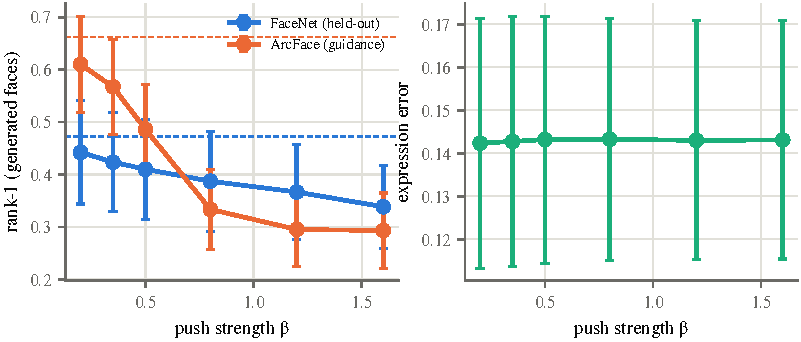
\includegraphics[width=\linewidth]{generated/e3_contribution/fig-e3-p2-curve}
\caption{E3c: rank-1 (FaceNet, ArcFace) e erro de expressão contra $\beta$; tracejado: mix nativo.}
\end{figure}

\subsection{Políticas (E3e)}
\begin{itemize}
\item Vídeo final, sobre P2 $\beta$ 1,2: P2 \result{e3e/pooled/p2/facenet_final.rank1}; \emph{hide-low} \result{e3e/pooled/hide-low/facenet_final.rank1}; \emph{gate} \result{e3e/pooled/gate/facenet_final.rank1}; ambos excluem zero.
\item Gerados: \emph{gate} \result{e3e/pooled/gate/anonymized}; \emph{hide-low} \result{e3e/pooled/hide-low/anonymized}.
\item Verificação: \emph{gate} \result{e3e/pooled/gate/facenet_final.verified} (a menor); \emph{hide-low} \result{e3e/pooled/hide-low/facenet_final.verified}.
\item Utilidade dos rostos mostrados: inalterada.
\end{itemize}

\subsection{P1 (E3g), negativo}
\begin{itemize}
\item FaceNet rank-1: \result{e3g/pooled/P1-c-0.1-+-P2/facenet.rank1} contra \result{e3g/pooled/P2/facenet.rank1} (P2 só); $\Delta$ \result{e3g/pooled/P1-c-0.1-+-P2/delta-facenet.rank1}~$\pm$~\result{e3g/pooled/P1-c-0.1-+-P2/delta-facenet.rank1.ci}, inclui zero.
\item Dentro do passo base, funciona: cosseno $\hat{x}_0$--real \result{e3g/pooled/guided-cos.p1-c0.1.first} $\to$ \result{e3g/pooled/guided-cos.p1-c0.1.last} (\result{e3g/pooled/guided-cos.p1-c0.1.identities} identidades).
\item Na imagem de identidade final: \result{e3g/pooled/identity-cos.p1-c0.1} com P1 contra \result{e3g/pooled/identity-cos.plain} sem (mediana pareada \result{e3g/pooled/identity-cos.p1-c0.1.paired-median}).
\item Onde se perde: último passo base, decodificação e refiner (img2img só com o prompt). O resto chega à troca só pelo embedding, que P2 já empurra.
\end{itemize}

\subsection{P3 (E3f), negativo}
\begin{itemize}
\item $\Delta$ FaceNet rank-1: \result{e3f/pooled/P3-tau-0.0/delta-facenet.rank1} ($\tau = 0$), \result{e3f/pooled/P3-tau--0.2/delta-facenet.rank1} ($\tau = -0{,}2$).
\item CIAGAN puro já perto do acaso: \result{e3f/pooled/ciagan/facenet.rank1}.
\item \emph{Hinge} ativa em \result{e3f/pooled/P3-tau-0.0/push.active} ($\tau = 0$) e \result{e3f/pooled/P3-tau--0.2/push.active} ($\tau = -0{,}2$) dos rostos.
\item Cosseno: \result{e3f/pooled/P3-tau-0.0/push.cos-start} $\to$ \result{e3f/pooled/P3-tau-0.0/push.cos-end}; massa no código da seed \result{e3f/pooled/P3-tau-0.0/push.p-seed}.
\item O otimizador não move o código: penalidade do pseudônimo, gradiente plano do softmax, pouca variação de identidade dentro do casco.
\end{itemize}

\section{E5: custo}
\begin{itemize}
\item ms por rosto: \emph{ref-cpu} \result{e5/pooled/ref-cpu/ms-per-face}; \emph{ref} \result{e5/pooled/ref/ms-per-face}.
\item Segmentação de cabeça: \result{e5/pooled/ref-cpu/stage-seg-ms}\,ms na CPU contra \result{e5/pooled/ref/stage-seg-ms}\,ms na GPU. Sem diferença pareada em privacidade ou utilidade.
\item Estágios por rosto gerado (\emph{ref}): GFPGAN \result{e5/pooled/ref/stage-gfpgan-ms}\,ms; landmarks \result{e5/pooled/ref/stage-landm-ms}\,ms; troca \result{e5/pooled/ref/stage-swap-ms}\,ms. PNG e RPC $\sim$10\,ms (medido no profiling).
\item GFPGAN desligado:
  \begin{itemize}
  \item \result{e5/pooled/enh-off/ms-per-face}\,ms por rosto (\result{e5/pooled/enh-off/speedup}$\times$);
  \item $\Delta\kappa$ nos rostos mostrados nos dois braços \result{e5/pooled/enh-off/delta-kappa}~$\pm$~\result{e5/pooled/enh-off/delta-kappa.ci} ($\kappa$ \result{e5/pooled/ref/emotion_kappa_video} $\to$ \result{e5/pooled/enh-off/emotion_kappa_video});
  \item expressão $\Delta$ \result{e5/pooled/enh-off/delta-expr};
  \item \emph{gate} rejeita \result{e5/pooled/enh-off/gated-share} contra \result{e5/pooled/ref/gated-share}; ocultos \result{e5/pooled/enh-off/hidden-share} contra \result{e5/pooled/ref/hidden-share};
  \item rank-1 $\Delta$ \result{e5/pooled/enh-off/delta-fn-r1} (inclui zero): o \emph{gate} absorve o vazamento ocultando rostos.
  \end{itemize}
\item GFPGAN só $\ge 96$\,px: igual a desligado (poucos rostos grandes).
\item Amostragem fixa a cada 3: \result{e5/pooled/every3/speedup}$\times$, nenhuma diferença pareada exclui zero.
\item Adaptativa $\tau = 0{,}08$:
  \begin{itemize}
  \item gera \result{e5/pooled/adapt-0.08/generated-share} dos rostos; \result{e5/pooled/adapt-0.08/speedup}$\times$;
  \item movimento $\Delta$ \result{e5/pooled/adapt-0.08/delta-motion}; $\Delta\kappa$ \result{e5/pooled/adapt-0.08/delta-kappa} (ambos melhoram);
  \item rank-1 $\Delta$ \result{e5/pooled/adapt-0.08/delta-fn-r1}.
  \end{itemize}
\item GPU-horas por hora de aula (30\,fps, 20 rostos por quadro): \emph{ref-cpu} \result{e5/pooled/ref-cpu/class-hours}; \emph{ref} \result{e5/pooled/ref/class-hours}; adaptativa 0,08 \result{e5/pooled/adapt-0.08/class-hours}.
\item O mesmo pipeline no vídeo composto (\emph{ref}): FaceNet rank-1 \result{e5/pooled/ref/facenet_video.rank1}, contra \result{e3e/pooled/gate/facenet_final.rank1} na visão de vídeo final do E3 (compressão e reaproveitamento como mostrados).
\end{itemize}

\begin{table}[ht]\centering
\caption{E5: custo por braço (gerados, ms por rosto, estágios, aceleração, GPU-horas por hora de aula).}
\input{generated/e5_cost/tab-e5-cost}
\end{table}

\begin{table}[ht]\centering
\caption{E5: cada braço menos \emph{ref}, nos mesmos rostos; * = intervalo exclui zero.}
\input{generated/e5_cost/tab-e5-paired}
\end{table}

\begin{figure}[ht]\centering
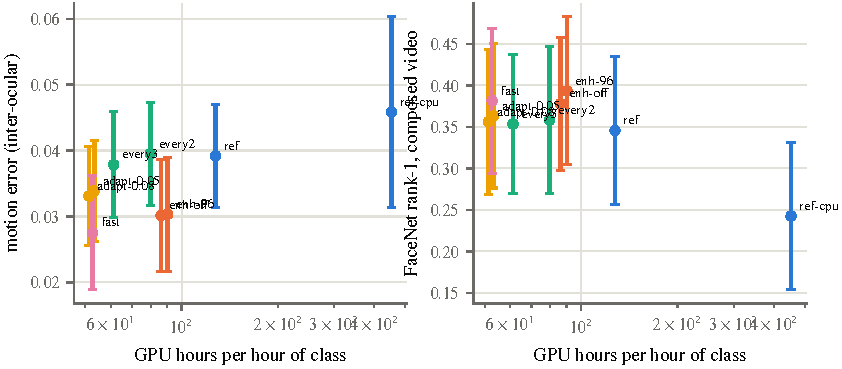
\includegraphics[width=\linewidth]{generated/e5_cost/fig-e5-tradeoff}
\caption{E5: GPU-horas por hora de aula, FaceNet rank-1, $\kappa$ e movimento no vídeo composto, por braço.}
\end{figure}
		% resultados E0--E5
\chapter{Pipeline final e discussão}
\label{cap:discussao}

% Rascunho em tópicos (2026-10-22).
% 2026-10-29 (parecer de orientação): ameaças à validade; alegações recalibradas
% (desidentificação; "sem diferença significativa" em vez de "sem perda"); β escolhido
% nos mesmos vídeos, com LOVO ao lado.
% 2026-10-30 (análise crítica): comparação com o BLANKET liberado pelo par privacidade x
% cobertura; empate de expressão com o GANonymization; ameaças: piloto, track como
% identidade, recall, galeria, atacantes por track e ciente do empurrão.

\section{Pipeline final}
\begin{enumerate}
\item Estágio~1: SCRFD-10GF a 0,1, rastreador estilo ByteTrack, pós-passe de recall.
\item BLANKET com a detecção do Estágio~1 na troca, identidade do track (C2) como alvo, P2 $\beta = 1{,}2$, processo principal na GPU.
\item \emph{Privacy gate} no limiar do vídeo a FAR 1\%.
\item Amostragem adaptativa: $\tau_a = 0{,}08$ IOD, máximo de 6 quadros.
\item Composição \emph{fail-closed}, com rejeição de saídas que não alteram o rosto (2026-10-29).
\end{enumerate}

\section{Números do pipeline final}
\begin{itemize}
\item Sem amostragem (E3e): vídeo final rank-1 \result{e3e/pooled/gate/facenet_final.rank1} (macro \result{derived/gate-final/macro}; \result{derived/gate-final/x-chance-min}$\times$--\result{derived/gate-final/x-chance-max}$\times$ o acaso); verificação \result{e3e/pooled/gate/facenet_final.verified}; gerados \result{e3e/pooled/gate/anonymized}.
\item Utilidade (rostos gerados): expressão \result{e3e/pooled/gate/expression}; pose \result{e3e/pooled/gate/pose_err}\textdegree; $\kappa$ \result{e3e/pooled/gate/emotion_kappa}.
\item No vídeo composto, com amostragem adaptativa (E5): rank-1 \result{e5/pooled/adapt-0.08/facenet_video.rank1}; \result{e5/pooled/adapt-0.08/class-hours} GPU-horas projetadas por hora de aula (laço por rosto).
\end{itemize}

\section{Escolhas}
\begin{itemize}
\item $\beta = 1{,}2$, não 1,6: ArcFace satura em 1,2; $\kappa$ maior; políticas medidas em 1,2. Escolhido nos mesmos três vídeos; LOVO escolhe 1,6, 1,6 e 1,2 (Tabela~\ref{tab:derived-lovo}).
\item $\beta$ 1,2 fica no lado da antípoda (cosseno \result{derived/p2geom/b-1.2/cos-real} com a identidade real); se o rank inverso mostrar reversibilidade, o ponto de operação passa a $\beta \approx$ \result{derived/p2geom/orthogonal-beta} (pendente).
\item \emph{Gate}, não \emph{hide-low}: mesmo rank-1 com metade dos rostos ocultos e menor verificação.
\item Alvo: a média simples estima tão bem quanto a ponderada (E3a); como alvo não há diferença (E3d).
\item GFPGAN ligado: parte da privacidade.
\item P1 e P3 fora.
\item SCRFD-10GF: licença verificada; YOLO-FaceV2-s tem mais recall, licença não verificada.
\end{itemize}

\section{Variante que prioriza o comportamento}
\begin{itemize}
\item GFPGAN desligado: $\kappa$ \result{e5/pooled/enh-off/emotion_kappa_video} (o maior de qualquer método medido).
\item Custo: \result{e5/pooled/enh-off/hidden-share} dos rostos ocultos; verificação \result{e5/pooled/enh-off/facenet_video.verified} contra \result{e5/pooled/ref/facenet_video.verified}.
\item Ocultar conta como privacidade: comparar pelo par (rank-1 entre os rostos mostrados, parcela mostrada).
\item Escolha depende do estudo: todos os rostos visíveis ou expressões fiéis.
\end{itemize}

\section{Leitura}
\begin{itemize}
\item Contra o BLANKET do código liberado, pelo par privacidade $\times$ cobertura (Figura~\ref{fig:derived-frontier}): face sintética em \result{derived/frontier/e5-ref/share} dos rostos contra \result{derived/frontier/e2-blanket/share}, com rank-1 entre eles de \result{derived/frontier/e5-ref/rank1} contra \result{derived/frontier/e2-blanket/rank1}. No rank-1 do vídeo final o BLANKET liberado fica abaixo (\result{e2/pooled/blanket/facenet_final.rank1} contra \result{e3e/pooled/gate/facenet_final.rank1}), porque 72\% dos seus rostos viram elipse cinza. Comparar o vídeo final do pipeline com a visão ``passthrough como vazamento do BLANKET (\result{e2/pooled/blanket/facenet.rank1}) misturaria visões (corrigido em 2026-10-30).
\item Acima do acaso e do blur (\result{e2/pooled/blur/facenet_final.rank1}); blur não carrega comportamento. Outro ponto do compromisso, não dominância. No vídeo final, blur, mosaico, CIAGAN e GANonymization têm rank-1 menor que o do pipeline.
\item Contra o GANonymization: mesmo erro de expressão, pose e $\kappa$ melhores, cobertura maior, reidentificação maior nos rostos gerados (\result{e3c/pooled/b-1.2/facenet.rank1} contra \result{e2/pooled/ganonymization/generated/facenet.rank1}).
\item Medir só os rostos que o método escolhe substituir, ou só o que ele publica, distorce a privacidade.
\item Avaliar só com o reconhecedor usado na otimização superestima o ganho (ArcFace contra FaceNet).
\item Rostos grandes vazam: a troca preserva o formato do rosto alvo \citep{bondalakunta}. Rosto do professor: maior risco; política por tamanho (trabalho futuro).
\item O enhancer re-renderiza o rosto: apaga identidade residual e expressão juntas.
\item Gerar menos quadros quase não custa nada: segurar o rosto quando o real está parado tira o tremor da troca.
\end{itemize}

\section{Ameaças à validade}
\label{sec:ameacas-validade}
\begin{itemize}
\item Interna:
  \begin{itemize}
  \item $\beta$, política do \emph{gate}, $\tau_a$ e parâmetros do pós-passe escolhidos nos mesmos vídeos avaliados; sem conjunto de teste;
  \item mitigação: LOVO para $\beta$ (direção mantida, magnitude não); pipeline congelado para avaliação em vídeos novos;
  \item saída sem troca registrada como gerada (\emph{fail-open}) nos braços sem \emph{gate}; corrigida, frequência não medida.
  \item fonte da troca possivelmente um vizinho real em parte das identidades exportadas (rosto de maior score no crop de contexto); corrigida em 2026-10-30, frequência não medida;
  \item piloto exploratório nos mesmos vídeos antes de fixar os critérios (P2 visto em 2026-09-26, critérios em 2026-09-29); pipeline final escolhido depois da campanha;
  \item identidade de referência = track do rastreador (guloso, sem modelo de movimento): fragmentação conta acerto como privacidade; auditoria de pares candidatos implementada, conferência pendente.
  \end{itemize}
\item Externa:
  \begin{itemize}
  \item três clipes, 29,1\,s, 59 tracks; demo3 = 54\% dos rostos;
  \item vídeos públicos, não consentidos, sem crianças identificadas como tal; validade em crianças não demonstrada;
  \item custo projetado de 29\,s para 1\,h.
  \item galeria do mesmo clipe de poucos segundos; atacante com foto de outra sessão não medido;
  \item recall sem anotação: o YOLO-FaceV2-s acha 25\% a 37\% mais caixas por quadro; rostos perdidos pelo detector saem reais.
  \end{itemize}
\item De construto:
  \begin{itemize}
  \item privacidade = reidentificação automática do miolo do rosto, galeria fechada, atacante ingênuo (Seção~\ref{sec:ameaca});
  \item unidade = quadro; atacante por pessoa (rank-1 por track) e atacante ciente do empurrão (rank inverso) implementados, pendentes;
  \item erro de expressão por landmarks favorece a troca, que mantém a geometria do rosto alvo por construção;
  \item avaliador fraco no demo1 (TAR FaceNet \result{e0/demo1/facenet.tar} nos rostos reais);
  \item probes de utilidade não validados em rostos de 30--80\,px; $\kappa \le 0{,}2$ na maioria dos braços;
  \item analisabilidade pedagógica (O3) não medida; proxy de orientação pendente;
  \item rosto oculto conta como não reidentificado.
  \end{itemize}
\item De conclusão:
  \begin{itemize}
  \item ``sem custo de utilidade'' = sem diferença significativa com 59 tracks (baixo poder), não equivalência; TOST não feito;
  \item comparações múltiplas: Holm por família implementado; valores ajustados pendentes da próxima exportação;
  \item agregado ponderado por rosto; macro-média e valores por vídeo ao lado.
  \end{itemize}
\end{itemize}

\section{O que o trabalho pode afirmar (e o que não)}
\begin{itemize}
\item Pode: a ordem dos métodos depende da visão medida; o pipeline cobre muito mais rostos que o BLANKET liberado com menos reidentificação por rosto mostrado; P2 reduz a reidentificação de forma significativa num avaliador não usado na otimização, monotônica no agregado, com direção mantida no LOVO; o mix nativo não faz nada mensurável; P1 e P3 não funcionam neste pipeline, por razões da arquitetura (diagnóstico); o GFPGAN faz trabalho de privacidade; amostragem adaptativa reduz o custo do laço 2,5$\times$ sem diferença pareada significativa.
\item Não pode: anonimização no sentido da LGPD (identificadores fora do rosto permanecem); mais privacidade que censura ou GANs no vídeo final; preservação de expressão (erro $\approx 4\times$ o piso, igual ao GANonymization); que o P2 seja irreversível (rank inverso pendente); reidentificação por aluno (pendente); ``primeiro'' empurrão contra a identidade real (NullFace, FAMS, Reverse Personalization, mix do FaceFusion); C2 como mecanismo novo (NAN, QAN, Zhu et al.); privacidade formal; validade em crianças; generalização para além dos três vídeos.
\end{itemize}
		% pipeline final e discussão
\chapter{Limitações, ética e conclusão}
\label{cap:conclusao}

% Rascunho em tópicos (2026-10-22).
% 2026-10-29 (parecer de orientação): identificadores fora do rosto, origem dos vídeos,
% CEP, fail-open, escopo do custo; E4-lite, política por tamanho e parrot como futuros.

\section{Limitações}
\begin{itemize}
\item Três vídeos de demonstração públicos na internet (29,1\,s); não é um conjunto consentido de crianças.
\item Hiperparâmetros escolhidos nos mesmos vídeos (Seção~\ref{sec:ameacas-validade}).
\item Atacante ingênuo: sem \emph{parrot attack} (reconhecedor retreinado nos rostos anonimizados) \citep{hanisch}.
\item Identificadores fora do rosto não tratados: cabelo, contorno da cabeça, orelhas, roupa, lugar na sala, corpo, voz.
\item Sem avaliação humana de analisabilidade pedagógica.
\item Sem análise de equidade demográfica.
\item Olhar (\emph{gaze}) não medido.
\item Rostos nunca detectados não são ocultados; taxa residual depende de anotação (pendente).
\item Saídas sem troca registradas como geradas (\emph{fail-open}): corrigido em 2026-10-29; frequência nas execuções existentes não medida.
\item Dois reconhecedores; não é garantia formal.
\item Custo: \result{e5/pooled/adapt-0.08/class-hours} GPU-horas por hora de aula, projeção só do laço por rosto; tempo ponta a ponta não medido; só \emph{offline}.
\item Componentes apenas para pesquisa não comercial (Apêndice~\ref{ap:licencas}).
\end{itemize}

\section{Ética e LGPD}
\begin{itemize}
\item Rosto: dado biométrico; etnia: dado sensível; menores: consentimento de um dos pais \citep{lgpd}.
\item Resultado: desidentificação facial, não dado anonimizado (art.~12); o vídeo processado continua dado pessoal.
\item Embeddings reais só em memória; scratch da ponte apagado também em SIGTERM e SIGHUP; crops de rostos não substituídos não são gravados (2026-10-29).
\item Resíduos com fundo real (crops gerados, imagens de identidade, vídeos compostos): removidos com \texttt{experiments/purge.sh} após a exportação.
\item Nenhum quadro de pessoa real no texto; exemplos qualitativos só com rostos sintéticos ou adultos consentidos.
\item Imagens de identidade do SDXL não contam como sintéticas para publicação (cosseno \result{e3g/pooled/identity-cos.plain} com a pessoa real).
\item Vídeos: públicos na internet; fonte, licença e termos por vídeo pendentes de registro.
\item Pendente: consulta ao CEP da UFPR (via orientador e coordenação). Plano B: gravações próprias com adultos voluntários e termo de uso de imagem.
\item Base legal a validar com o orientador e o CEP (não afirmada): LGPD art.~7º, IV e art.~11, II, c, tratamento por órgão de pesquisa para estudos, garantida a anonimização sempre que possível \citep{lgpd}. Esta tese processou biometria de pessoas que não consentiram; o registro da fonte de cada vídeo e a consulta ao CEP são condição para a defesa.
\item Cópias locais dos vídeos e resultados fora do servidor: apagadas (2026-10-29).
\end{itemize}

\section{Trabalhos futuros}
\begin{itemize}
\item Rodar no servidor o que já está implementado: rank inverso, rank-1 por track, rank-1 entre rostos mostrados, auditoria de identidades, $\kappa$ de orientação, estratos por tamanho, Holm; conferir à mão os pares de tracks candidatos e as caixas extras do YOLO-FaceV2-s.
\item Braço $\beta \approx c$ (ortogonal): remove a componente real sem ir para a antípoda.
\item E4-lite, banco de identidades: identidades geradas por prompt genérico, sem condicionar na imagem real e sem inferir atributos; remove a rota de vazamento da imagem de identidade e o custo de difusão por track (1 a 2 dias).
\item E4, identidade só por texto:
  \begin{itemize}
  \item atributos grosseiros (faixa etária, gênero aparente, óculos, cabelo) $\to$ template $\to$ texto-para-imagem, sem ver o rosto real \citep{lee2026,deepprivacy};
  \item remove a rota de vazamento da imagem de identidade (cosseno \result{e3g/pooled/identity-cos.plain}); a troca continua vazando forma;
  \item sem tom de pele ou etnia no vocabulário (LGPD art.~11); validar com compliance e comitê de ética;
  \item riscos: viés e homogeneização do texto-para-imagem, memorização, reidentificação pelo próprio texto.
  \end{itemize}
\item Política por tamanho do rosto: $\beta$ maior, \emph{gate} mais estrito ou ocultação para rostos $\ge 96$\,px (professor).
\item Atacante ciente simplificado (\emph{parrot}: galeria também substituída) \citep{hanisch}.
\item Testes de equivalência (TOST) com margens no piso de ruído.
\item Avaliação em vídeos novos, separados, com o pipeline congelado.
\item Custo da identidade: offload por modelo no lugar do sequencial, sem refiner, LCM-LoRA em 4--5 passos \citep{lcmlora}, DeepCache \citep{deepcache}.
\item Custo por rosto: TensorRT fp16, lotes por quadro, vários workers por GPU, divisão do vídeo entre GPUs; tempo ponta a ponta por estágio.
\item P1 no refiner, ou sem refiner.
\item $\beta = 1{,}6$ com \emph{gate}; \emph{hide-low} com \emph{gate}.
\item Ground truth de exposição (rostos nunca detectados, trocas de ID); decisão final do detector.
\item Equidade demográfica; avaliação humana com gravação consentida.
\end{itemize}

\section{Conclusão}
\begin{itemize}
\item Substituir rostos com identidade sintética fixa por track, empurrada para longe da identidade real, reduz a reidentificação facial automática e mantém expressão e pose melhor que censura e GANs.
\item É desidentificação facial parcial (3--9$\times$ o acaso por vídeo), não anonimização; o ganho sobre o BLANKET liberado é cobertura com menos reidentificação por rosto mostrado, não privacidade maior que censura no vídeo final.
\item Não é mais privado que blur; é outro ponto do compromisso.
\item Emoção não é preservada por nenhum método.
\item A privacidade de um método depende de quais rostos são medidos; medir o vídeo final.
\item Custo: \result{e5/pooled/adapt-0.08/class-hours} GPU-horas por hora de aula só no laço por rosto (O4 refutado); viável para estudos de poucas horas de vídeo, não para acervos de um semestre.
\end{itemize}
		% limitações, ética, conclusão

%=====================================================

% ATENÇÃO:
% - o estilo da bibliografia é definido no arquivo packages.tex
% - evite usar \cite{}; prefira \citep{} e \citet{}

% base de bibliografia (arquivo .bib do BibTeX)
\bibliography{referencias}
%\bibliography{file1,file2,file3} % se tiver mais de um arquivo BibTeX

%=====================================================

% inclusão de apêndices
\appendix
\chapter{Componentes e licenças}
\label{ap:licencas}

% Verificado em 2026-10-21 nas páginas dos projetos.

\begin{itemize}
\item SCRFD, ArcFace \texttt{w600k\_r50}, \texttt{2d106det}, \texttt{1k3d68}, \texttt{genderage} (pacote \texttt{buffalo\_l}): código MIT; modelos apenas para pesquisa não comercial \citep{insightface}.
\item \texttt{inswapper\_128}: apenas pesquisa não comercial; licenciamento comercial via InsightFace (desde 2025-11).
\item BLANKET: GPL-3.0; isolado em processos próprios na ponte \citep{blanket}.
\item FaceFusion: OpenRAIL-AS \citep{facefusion}.
\item GFPGAN: Apache-2.0, com partes não comerciais (StyleGAN2 da NVIDIA; DFDNet CC BY-NC-SA); treinado em FFHQ (CC BY-NC-SA 4.0) \citep{gfpgan,ffhq}.
\item SDXL inpainting, refiner e ControlNets: licenças dos respectivos cards (OpenRAIL++).
\item CIAGAN: MIT \citep{ciagan}.
\item GANonymization: MIT \citep{hellmann}.
\item facenet-pytorch: MIT; pesos VGGFace2 \citep{facenetpytorch,vggface2}.
\item HSEmotion: código Apache-2.0; pesos sem licença declarada; reporta resultados em AffectNet, cujos termos permitem só pesquisa \citep{hsemotion,affectnet}.
\item YOLO-FaceV2: README diz MIT, mas deriva do YOLOv5 (AGPL-3.0); não verificado \citep{yolofacev2}.
\item Conclusão: uso acadêmico apenas; uso comercial exigiria trocar \texttt{inswapper}, os modelos do InsightFace e o GFPGAN.
\end{itemize}
		% componentes e licenças
\chapter{Registro de decisões}
\label{ap:decisoes}

% Resumo de experiments/DECISIONS.md (1--52) e do log do vault (70-decisions).

\section{Detecção}
\begin{itemize}
\item 2026-08-06: o ``RetinaFace'' do \texttt{buffalo\_l} é SCRFD-10GF; texto corrigido.
\item 2026-09-18: detectores trocáveis; \texttt{onnxruntime-gpu} (CUDA 12): SCRFD de 0,4 para 9,3 quadros/s.
\item 2026-09-30: limiar 0,1 (era 0,5 por bug); pós-passe de recall por padrão.
\item 2026-10-15: SCRFD-10GF mantido (licença do YOLO-FaceV2 não verificada).
\end{itemize}

\section{Geração}
\begin{itemize}
\item 2026-09-22/23: CIAGAN e GANonymization calibrados; GANs considerados esgotados (máscara só de rosto; qualidade do gerador).
\item 2026-09-23: Reverse Personalization descartado (sem crianças, sem vídeo).
\item 2026-09-24: BLANKET integrado em ponte isolada; prompt sem ``baby face''.
\item 2026-09-26: P2 funciona (FaceNet cai de forma monotônica com $\beta$).
\item 2026-09-30: troca usa o rosto do Estágio~1; detector permissivo para imagens de identidade.
\end{itemize}

\section{Avaliação}
\begin{itemize}
\item FaceNet como avaliador não usado na otimização; ArcFace ao lado.
\item APIs comerciais de reconhecimento: removidas (ética, LGPD).
\item \emph{Parrot attack}, ID-switch, avaliação humana, equidade: limitações.
\item Emoção como $\kappa$ (não concordância bruta).
\item McNemar substituído por teste de inversão de sinal por track (rostos de um track não são independentes).
\item Três visões de privacidade; vídeo composto no E5.
\item Critérios fixados antes de rodar (2026-09-29).
\end{itemize}

\section{Composição e dados}
\begin{itemize}
\item 2026-09-30: \emph{fail-closed}; colar só pixels alterados; elipse cinza em vez de blur.
\item 2026-10-20/21: crops com fundo real e rascunhos de identidade apagados após uso; arquivos antigos apagados.
\end{itemize}

\section{Contribuição e pipeline final}
\begin{itemize}
\item 2026-09-24: contribuição escolhida: empurrão de identidade em três pontos (P1, P2, P3) contra a identidade real do track (C2).
\item 2026-10-15: P1 e P3 negativos; pipeline final = E3e \emph{gate}.
\item 2026-10-21: correções da auditoria (split do E3a, $p$ ponderado, $\kappa$ no vídeo composto, tempo em regime).
\item 2026-10-21: E5; processo principal na GPU e amostragem adaptativa entram no pipeline final; GFPGAN mantido.
\end{itemize}
		% registro de decisões
\chapter{Infraestrutura e reprodução}
\label{ap:reproducao}

% 2026-10-29: testes, proveniência completa, pendências de reprodução (parecer, I7).

\begin{itemize}
\item Servidor: serra1 (UFPR), 2$\times$ NVIDIA RTX A5000 24\,GB, 48 núcleos, 125\,GB RAM, compartilhado. Indisponível desde 2026-10-21 (isolado pela administração).
\item Ambiente: Python com \texttt{uv}; \texttt{onnxruntime-gpu} 1.20.2 (CUDA 12); dois venvs isolados para a ponte do BLANKET.
\item Ponte: repositório \texttt{blanket-anonymizer-bridge} (servidores de identidade e de troca, RPC por socket Unix).
\item Experimentos: \texttt{experiments/e0..e5}, cada um com \texttt{config.toml}, \texttt{run.py}, README.
  \begin{itemize}
  \item \texttt{run\_all.sh} (\texttt{--only}, \texttt{--resume}); \texttt{smoke.sh};
  \item proveniência por execução (commit, hashes das entradas, comandos);
  \item exportação para o texto: \texttt{export\_paper.sh}, que leva tabelas, figuras e chaves para \texttt{paper/generated} e roda \texttt{derived.py} e \texttt{tables\_pt.py};
  \item \texttt{SOURCES.md}: commit do projeto e da ponte (com estado sujo), versões de Python e torch, hash do \texttt{uv.lock} (2026-10-29);
  \item \texttt{check\_latex.sh}: tudo compila e cabe em 160\,mm;
  \item \texttt{purge.sh}: remove resíduos com pessoas reais após a exportação.
  \end{itemize}
\item Testes unitários: \texttt{tests/} (pytest), só com arrays sintéticos: composição \emph{fail-closed}, políticas de geração, erro de landmarks, rastreador, pós-passe de recall, estatística e chaves; 45 testes, executados no servidor macalan (UFPR) em 2026-10-29.
\item Tempos: E0 61\,min; E1 19\,min; E2 $\sim$1 dia; E3 $\sim$50\,h; E5 8,2\,h.
\item Identidades SDXL congeladas em cache por vídeo; seeds determinísticas por track (dependem do caminho do vídeo).
\item Execuções exportadas em 5 commits diferentes; E1 com árvore suja (\texttt{SOURCES.md}).
\item Pendente (servidor): push dos commits da ponte \texttt{f376d0b}, \texttt{3004a3a}, \texttt{16cf02d} e fixação no \texttt{NOTICE}; E0 e E1 de novo no commit final ($\approx$80\,min); \texttt{smoke.sh} após a limpeza; tag \texttt{tcc-defesa}.
\item Código: \texttt{github.com/ld-wg/lose-the-faces-keep-the-lesson}, PR \#12 (campanha de resultados) e PR de fechamento do parecer (\texttt{feature/wrap-up-review}).
\end{itemize}
		% infraestrutura e reprodução
\chapter{Correções do parecer de orientação (2026-10-29)}
\label{ap:parecer}

% Fonte: research/next-steps/parecer-orientador-2026-10-29.md (vault).
% Código: branch feature/wrap-up-review; decisões 53--60 em experiments/DECISIONS.md.
% Estado: feito = no código ou no texto; pendente (servidor) = depende do serra1,
% indisponível desde 2026-10-21; pendente (orientador/autor) = decisão fora do código.

\section{Críticos}
\begin{itemize}
\item C1, procedência e ética dos dados.
  \begin{itemize}
  \item Feito: origem registrada como ``vídeos públicos na internet'' (Seção~\ref{cap:experimentos}); cópias locais de vídeos e resultados apagadas; tratamento de dados corrigido (Seção~\ref{cap:metodo}).
  \item Pendente (autor): fonte, licença e termos de cada vídeo.
  \item Pendente (orientador): consulta ao CEP; plano B com gravações próprias consentidas.
  \end{itemize}
\item C2, tamanho e representatividade dos dados.
  \begin{itemize}
  \item Feito: valores por vídeo, macro-média e múltiplo do acaso (Tabela~\ref{tab:derived-chance}); duração e participação de cada vídeo no agregado; ameaça à validade externa (Seção~\ref{sec:ameacas-validade}).
  \item Pendente: mais dados; segundo reconhecedor não usado na otimização.
  \end{itemize}
\item C3, hiperparâmetros escolhidos nos dados de avaliação.
  \begin{itemize}
  \item Feito: LOVO para $\beta$ (Tabela~\ref{tab:derived-lovo}); ameaça à validade interna declarada.
  \item Pendente: vídeos de teste separados com o pipeline congelado.
  \end{itemize}
\item C4, modelo de ameaça e alegação de anonimização.
  \begin{itemize}
  \item Feito: modelo de ameaça (Seção~\ref{sec:ameaca}); alegação trocada para desidentificação facial em resumo, abstract, palavras-chave, introdução, discussão e conclusão; identificadores fora do rosto nas limitações.
  \item Pendente: \emph{parrot attack} (trabalho futuro); título (orientador).
  \end{itemize}
\item C5, furo na garantia \emph{fail-closed}.
  \begin{itemize}
  \item Feito: fração mínima de pixels alterados (1\%) no Estágio~2 e na composição; teste do invariante em quadros sintéticos.
  \item Pendente (servidor): frequência do \emph{fail-open} nas execuções existentes; anotação de rostos nunca detectados (\texttt{miss\_sheet}).
  \end{itemize}
\item C6, validade da utilidade.
  \begin{itemize}
  \item Feito: proxy de tarefa (orientação, $\kappa$) implementado; ``sem custo'' reescrito como ``sem diferença significativa''; ameaça à validade de construto.
  \item Pendente (servidor): $\kappa$ de orientação. Pendente: TOST; avaliação humana com gravação consentida; título (``Expression-Preserving'').
  \end{itemize}
\end{itemize}

\section{Importantes}
\begin{itemize}
\item I1, visões de privacidade inconsistentes: divergência declarada (Seção~\ref{cap:experimentos}). Pendente (servidor): E2/E3 com \texttt{--video-view}.
\item I2, ocultar infla a privacidade: declarado; par (rank-1 nos mostrados, parcela mostrada) na discussão.
\item I3, rostos grandes e o professor: estratos por tamanho no E3e e no E5 implementados; pendente (servidor). Política por tamanho: trabalho futuro.
\item I4, identidade sintética nasce do rosto real: declarado no modelo de ameaça; E4-lite como trabalho futuro.
\item I5, estatística: Holm por família; tabelas por vídeo e macro. Pendente: valores ajustados (próxima exportação); TOST.
\item I6, escopo da métrica de custo: definições de quadros/s (E2) e ms por rosto (E5) separadas; projeção rotulada; exclusões listadas. Pendente: tempo ponta a ponta por estágio.
\item I7, reprodutibilidade: \texttt{SOURCES.md} com commit da ponte, Python, torch e \texttt{uv.lock}; E5 aborta sem o cache do E3. Pendente (servidor): push da ponte, E0/E1 no commit final, tag \texttt{tcc-defesa}.
\item I8, sem testes: 45 testes unitários (\texttt{tests/}).
\item I9, dados reais persistidos: crops de rostos não substituídos não gravados; scratch apagado em SIGTERM e SIGHUP; \texttt{purge.sh}.
\item I10, novidade modesta: contribuições enquadradas como empíricas e de sistema (Seção~\ref{cap:intro}).
\item I11, dez divergências entre texto e código, corrigidas no texto:
  \begin{enumerate}
  \item dilatação só em tracks confirmados;
  \item rastreador sem modelo de movimento, associação gulosa;
  \item margem de contexto 0,8 do BLANKET não calibrada;
  \item $\beta = 0{,}35$ não equivale ao mix nativo (nativo normalizado $\approx 0{,}26$);
  \item re-detecção a 320\,px e corte 0,5;
  \item E1 com limiar 0,3;
  \item cache de identidades chaveado pela seed derivada do caminho;
  \item apagamento do scratch e dos crops descrito como realmente ocorre;
  \item GPU-horas sem detecção, pré-passe, identidades e composição;
  \item quadros/s do E2 com outra definição (tempo total).
  \end{enumerate}
\end{itemize}

\section{Menores e formato}
\begin{itemize}
\item Objetivos geral e específicos (O1--O4, com situação); classificação da pesquisa; desvios e Quadro~\ref{qua:desvios}.
\item ``Cap.'' substituído por ``Seção''.
\item Listas de figuras, tabelas e quadros ativadas; todo float com título acima, \texttt{\textbackslash label}, fonte abaixo e menção no texto.
\item Tabelas em português com vírgula decimal (\texttt{generated/<experimento>/pt}). Pendente (servidor): eixos das figuras em português.
\item Resumo e abstract em 3ª pessoa, parágrafo único, sem rótulos internos; palavras-chave com ``;'' e minúsculas.
\item Siglas completadas (CEP, CPU, GPU, EMA, IoU, LOVO, RMS, TCC, TOST, VAE e outras); $\tau$ desambiguado em $\tau_h$ e $\tau_a$; $\alpha_f$ na lista de símbolos.
\item Bibliografia: entradas ``verificar'' conferidas (LFW, FDDB, Deep OC-SORT, MPGD, HSEmotion, Fantômas); ``Disponível em'' e ``Acesso em'' nas referências online.
\item Restos do modelo removidos: \texttt{a1-exemplo}, \texttt{a2-exemplo}, \texttt{exemplo.c}, \texttt{exemplo-figura.pdf}, \texttt{main\_maziero.pdf}, \texttt{lipsum}; ficha catalográfica fora (não exigida para TCC); descrição do trabalho pelo modelo SiBi; ``Prof. Dr.'' no orientador.
\item README atualizado; \texttt{phase3\_temporal} removido; \texttt{fps} do \texttt{tracks.json}; código morto removido.
\item Pendente (orientador): idioma do documento e título; metas da hipótese.
\item Pendente (autor): agradecimentos e dedicatória; desenvolver os tópicos em parágrafos; diagrama do pipeline; geometria do P2.
\end{itemize}
		% correções do parecer de 2026-10-29

%=====================================================

\end{document}

%=====================================================
